% This is LLNCS.DEM the demonstration file of
% the LaTeX macro package from Springer-Verlag
% for Lecture Notes in Computer Science,
% version 2.4 for LaTeX2e as of 16. April 2010
%
\documentclass{llncs}
%
\usepackage{makeidx}  % allows for indexgeneration
\usepackage[pdftex]{graphicx}
\usepackage[cmex10]{amsmath}
\usepackage{algorithm}
\usepackage[noend]{algorithmic}
\usepackage{array}
\usepackage[tight,footnotesize]{subfigure}
\usepackage{booktabs}
\usepackage{threeparttable}

%
\begin{document}

%
\mainmatter              % start of the contributions
%
\title{DCF: A Dataflow Based Collaborative Filtering Training Algorithm}
%
\titlerunning{Hamiltonian Mechanics}  % abbreviated title (for running head)
%                                     also used for the TOC unless
%                                     \toctitle is used
%
\author{Xiangyu Ju \inst{1} \and Quan Chen \inst{1} \and
Zhenning Wang \inst{1} \and Minyi Guo \inst{1} \and Guang R. Gao \inst{2}}
%
\authorrunning{Xiangyu Ju et al.} % abbreviated author list (for running head)
%
%%%% list of authors for the TOC (use if author list has to be modified)
\tocauthor{Quan Chen, Zhenning Wang, Minyi Guo, Guang R. Gao }

\institute{Shanghai Jiao Tong University, Shanghai 200240, China,\\
\and
University of Delaware, Newark 19716, USA \\
\email{juxiangyu@sjtu.edu.cn}}

\maketitle              % typeset the title of the contribution
\vspace{-20pt}
\begin{abstract}
Emerging recommender systems often adopt collaborative filtering techniques to improve the recommending accuracy.  Existing collaborative filtering techniques are implemented with either Alternating Least Square (ALS) algorithm or Gradient Descent (GD) algorithm. However, both of the two algorithms  are not scalable because ALS suffers from high computational complexity and GD suffers from severe synchronization problem and tremendous data movement. To solve the above problem, we proposed a Dataflow-based Collaborative Filtering (DCF) algorithm.
More specifically, DCF exploits fine-grain asynchronous feature of dataflow model to minimize synchronization overhead; leverages mini-batch technique to reduce computation and communication complexities; uses dummy edge and multicasting techniques to avoid fine-grain overhead of dependency checking and reduce data movement. By utilizing all the above techniques, DCF is able to significantly improve the performance of collaborative filtering. Our experiment on a cluster with one master node and ten slave nodes show that DCF achieves 23x speedup over ALS on Spark and 18x speedup over gradient descent on Graphlab in public datasets.

%Collaborative filtering, widely used in big data applications, is a common technique in recommender systems. Most big data systems (e.g. Hadoop MR, Spark) use alternating least square (ALS) as the training algorithm for collaborative filtering. Due to the high computation complexity, ALS faces severe performance challenges when data become dramatically larger and sparser. Gradient descent is an alternative training algorithm with lower computation complexity. However, it requires fine-grain operations and large scale data movements. In this paper, we proposed dataflow based collaborative filtering (DCF) training algorithm. DCF exploits fine-grain asynchronous feature of dataflow model to achieve significant performance gain. With our method, the fine-grain overhead of dependency checking and high communication complexity can be optimized by dummy edge and multicasting techniques. We evaluate our algorithm and contrasts on 1 master + 10 slaves cluster. The experiment results show that DCF achieves 23x speedup over ALS on Spark and 18x speedup over gradient descent on Graphlab in public datasets.

\vspace{-5pt}

\begin{keywords} DCF; dataflow; collaborative filtering; gradient descent; asynchronous; fine-grain; parallel;
\end{keywords}
\vspace{-5pt}
\end{abstract}



%\vspace{-30pt}
\section{Introduction}
\vspace{-5pt}

With the immense growth of e-commerce and social network, recommender systems have shown increasing popularity and importance in recent years.
In order to achieve reasonable and user-specific recommendation, emerging recommender systems often adopt collaborative filtering technology that  extracts user characters from multiple aspects and makes recommendation by synthesizing all the characters. Collaborative filtering  can be implemented with either memory-based technique (e.g user based technique, item based technique)~\cite{MemoryBasedCF} or model-based technique (e.g., Alternating Least Square, and Gradient Descent)~\cite{towards}. Prior work~\cite{MF2009,recSurvey2013} has shown that collaborative filtering system is able to achieve better prediction accuracy adopting model-based techniques. To this end, well-known big data platforms (e.g. Hadoop \cite{Hadoop}, Spark \cite{SparkMllib}, Graphlab \cite{graphlab}) leverage model-based techniques, such as Alternating Least Square and Gradient Descent, to implement collaborative filtering.


However, recommender systems based on collaborative filtering suffer from poor performance in big data era. This is mainly because the volume of rating data from massive users increases dramatically but ALS and gradient descent perform poor when the data set is large. 
For ALS, its computation complexity increases with feature dimension quadratically~\cite{ibm2011} and this feature of ALS results in its poor scalability. For gradient descent, although it has a much lower computation complexity compared with ALS and outperforms ALS when the dataset is large~\cite{sgdKdd2015,sgdFast2015,ibm2011}, it still suffers from poor performance due to the following challenges. 
\textbf{First, gradient descent suffers from high communication complexity and the resulted network load becomes the new performance bottleneck. Second, individual operations of each data require fine-grain task scheduling and the scheduling overhead degrades the performance. Third, gradient descent is not able to fully utilize computing resources due to the high data sparsity.}

In order to solve the above challenges, we propose a {\it Dataflow-based Collaborative Filtering} (DCF) algorithm to improve the performance of distributed recommender systems. Dataflow~\cite{dataflow} is a parallel computation model that
supports asynchronous fine-grain task scheduling. Prior work~\cite{xxx} has shown that dataflow model is able to minimize communication complexity, reduce scheduling overhead, and increase resource utilization, especially in high data sparsity scenario. However, simply implementing gradient descent using dataflow model is not able to improve the performance of collaborative filtering, because the fine-grain dependency checking overhead and frequent data movements introduced by dataflow model becomes the new bottlenecks.
To this end, we further propose three optimizations, {\it dummy edge}, {\it multicasting}, and {\it mini-batch}, to minimize the extra overhead caused by dataflow model. More specifically, dummy edge technique exploits local data transmission in dataflow graph to reduce dependency checking overhead and unnecessary data movements. Multicasting technique avoids sending data to same node for reducing data movements. Mini-batch limits the dependency number of each feature vector to further reduce computation and communication complexity on algorithmic level. The main contributions of this paper are summarized as follows:

\vspace{-5pt}
\begin{itemize}
\item We design a dataflow-based collaborative filtering (DCF) algorithm that performs better than traditional gradient descent-based collaborative algorithm.
%We exploit the maximum parallelism of the algorithm without hurting convergence because of the deterministic feature of dataflow model.
% adding dummy edge optimization
\item We propose a dummy edge technique that handles fine-grain overhead of data dependency checking and reduce unnecessary data movements by exploiting  data locality.
\item We propose a multicasting technique that reduces the quantity of data transferred by network.
\item We apply an mini-batch technique that reduces computation and communication complexity of DCF algorithm.
\end{itemize}
\vspace{-5pt}
%\item  We apply mini-batch technique to DCF for reducing the computation and communication complexity of proposed algorithm with good convergence.

We have implemented DCF and evaluated it with public datasets. The experiment results demonstrate that DCF shows a 23X speedup over ALS on Spark and 18X speedup over gradient descent on Graphlab with similar accuracy.

\vspace{-10pt}

\section{Background \& Motivation}
\vspace{-10pt}

\label{sec:background}

Model-based collaborative filtering algorithms are adopted by most of emerging distributed recommender systems. As shown in Figure \ref{fig:MF}, model-based collaborative filtering algorithms convert a recommendation issue into a matrix factorization problem, transforming user-item-rating data into two separated matrixes which represent user features and item features. Predicting rates are made by the products of user feature vectors and item feature vectors.
ALS and gradient descent are two main training algorithms for model-based collaborative filtering.
\vspace{-5pt}

\begin{figure}[!htb]
\centering
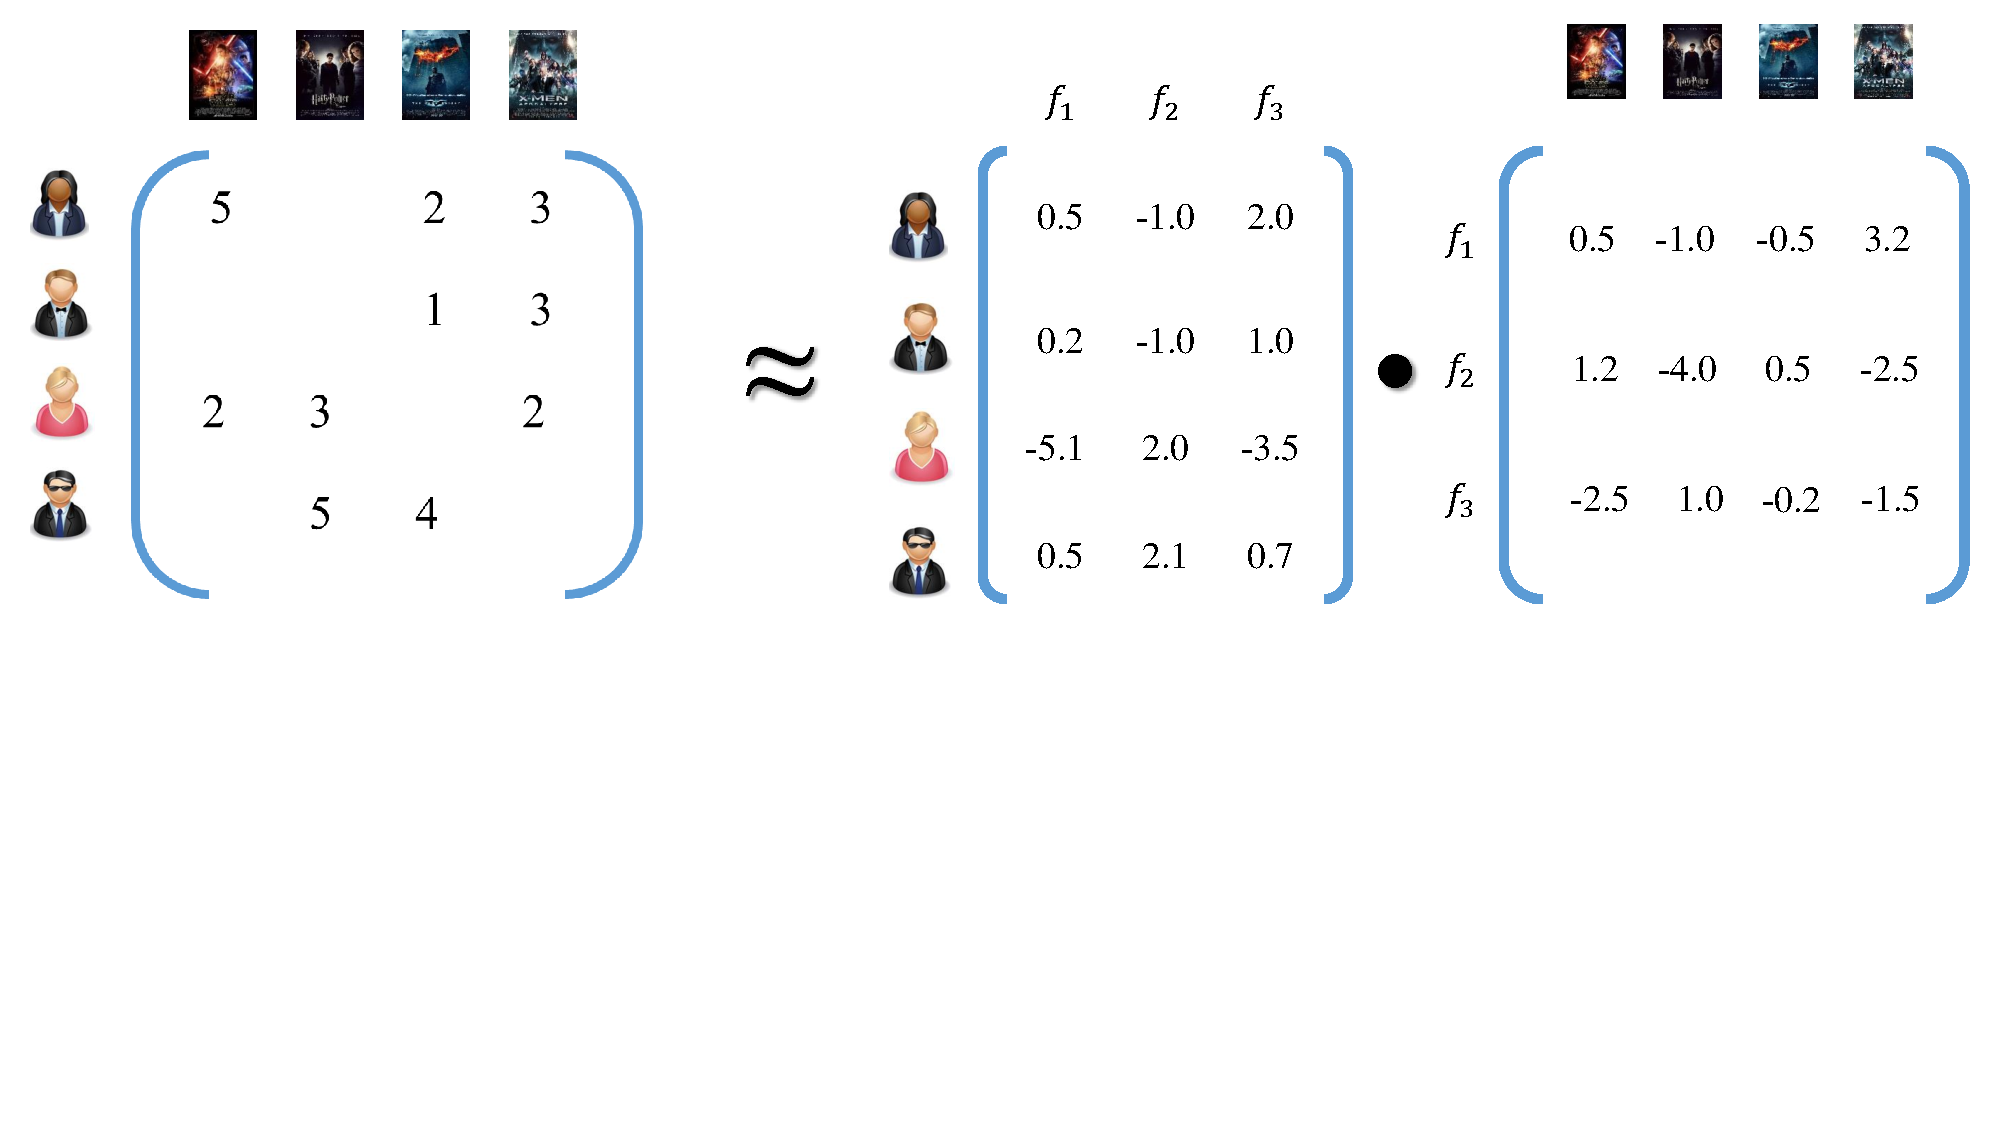
\includegraphics[width=3in]{pics/MFIntroduction.pdf}
\vspace{-60pt}
\caption{Model Based Collaborative Filtering}
\vspace{-15pt}
\label{fig:MF}
\end{figure}

%\vspace{-5pt}
\subsection{ALS \& Gradient Descent}
\label{sub:gd}
%\vspace{-5pt}

ALS \cite{ALS} converts the matrix factorization problem into a quadratic problem which can be optimally solved. According to the study of Gemulla et al. \cite{ibm2011}, the computation complexity of ALS is $O(k^3 + k^2(n_u + n_v) + kn_r)$ in one iteration, and it increases with feature dimension $k$ quadratically because user number $n_u$ or item number $n_v$ is much larger than $k$. ALS shows low performance in large scale datasets because of the high computation complexity.

Gradient descent is an alternating training algorithm for model based collaborative filtering. According to Eq. \ref{eq:gd1} and Eq. \ref{eq:gd2},
user feature vector $u_i$ or item feature vector $v_j$ can be updated by given ratings $r_{i,j}$ and dependent feature vectors where $\lambda$ represents the regularization parameter. The computation complexity of gradient descent is $O(k\bar{d}(n_u + n_v))$ in one iteration where $\bar{d}$ represents the average dependency number. Compared with ALS, gradient descent has a lower computation complexity. However, gradient descent also faces several challenges. Firstly, it requires fine-grain operations because each user feature vector $u_i$ or item feature vector $v_j$ can be updated individually and asynchronously. Secondly, high data sparsity causes load imbalance because dependency number of each feature vector varies in large scale. Thirdly, the communication complexity is $O(k\bar{d}(n_u + n_v))$ and it leads to high network load.
\vspace{-5pt}

\begin{equation}
\label{eq:gd1}
  u_i = u_i - \alpha (\sum_{r_{i,j} \neq 0}(u_i^Tv_j - r_{i,j})v_j + \lambda u_i)
\end{equation}
\vspace{-15pt}

\begin{equation}
\label{eq:gd2}
v_j = v_j - \alpha (\sum_{r_{i,j} \neq 0}(u^T_iv_j - r_{i,j})u_i + \lambda v_j)
\end{equation}


In order to develop high performance collaborative filtering algorithms, we select gradient descent as training algorithm for its low computation complexity. In addition, we need to find proper parallel model to solve its challenges. As a result, dataflow model is selected because it can partially solve the challenges of gradient descent.
%
%\begin{table}[!t]
%\caption{Computation and Communication Complexity Analysis of ALS and Gradient Descent}
%\label{tab:complexity}
%\centering
%\begin{tabular}{|c|c|c|}
%\hline
%& \textbf{Computation Complexity} & \textbf{Communication Complexity} \\
%\hline
%\textbf{ALS} & $O(k^3 + k^2 (n_u + n_v) + kn_r)$ & $O(k(n_v + n_u))$\\
%\hline
%\textbf{Gradient Descent} & $O(k\bar{d}(n_u + n_v))$ & $O(k\bar{d}(n_u + n_v))$\\
%\hline
%\end{tabular}
%\begin{tablenotes}
%\footnotesize
%\centering
%\item[1] user number($n_u$), item number($n_v$), rating number($n_r$), number of feature dimension ($k$), average dependency number($\bar{d}$)
%\end{tablenotes}
%\vspace{-15pt}
%\end{table}

\vspace{-10pt}
\subsection{Dataflow}
\vspace{-5pt}

Dataflow \cite{dataflow} is a data-driven computation model optimized for the execution of fine-grain parallel algorithms. Dataflow treats each computation as a separate task and the execution order is maintained by data dependency.
Dataflow model can be represented as directed acyclic graph (DAG) where nodes
represent computation and edges represent data dependencies.

The features of dataflow model can partially solve the challenges of gradient descent well. Fine-grain feature supports individual updating operations of each feature vector. Asynchronization supports sparse dependency well for fully utilizing computing resources. However, applying dataflow model to gradient descent is not straightforward because we need to solve the challenges of dataflow model as well. Fine-grain dependency checking overhead of each feature vector and frequent data movements are the main bottlenecks because of massive rating data.

In summary, we propose DCF algorithm with optimizations to solve the challenges of gradient descent and dataflow model.

\vspace{-10pt}
\section{DCF: Dataflow Based Collaborative Filtering Algorithm}
\vspace{-10pt}

In this section, we give a gradient descent algorithm based on dataflow execution model. Firstly, we demonstrate the working mechanism of dataflow execution model. Secondly, we transform gradient descent into dataflow graph and explain the working process of it. Thirdly, we propose optimizations to solve the challenges of dataflow model and gradient descent. Finally, we give a detailed DCF algorithm by applying proposed optimizations.
\vspace{-10pt}
\subsection{Dataflow Execution Model}
\vspace{-5pt}
%Introduce dataflow execution model briefly
In order to design dataflow algorithm, we introduce the working process of dataflow execution model. As shown in Figure \ref{fig:dataflowModel}, we give an example to explain dataflow execution model explicitly. The figure shows a snapshot of a simple computing progress which consists of several basic operator tasks. Dataflow execution model schedules and processes tasks generated by dataflow graph. Dataflow graph is a directed acyclic graph which edges represent data dependencies and nodes represent functions. The basic data structure transferred in dataflow graph is key-value pair. A task is composed of data from input edges with same key and function of the node. Once dependent data of one node is satisfied, corresponding tasks will be generated and pushed to task queue, such as $-$ task, $\sqrt{ }$ task and $\div$ task. As the input data of $+$ node have different keys, the task will be not generated until dependent data with same key arrive. Processing elements (PE) will fetch new tasks in task queue until tasks are finished.

\begin{figure}[!t]
\centering
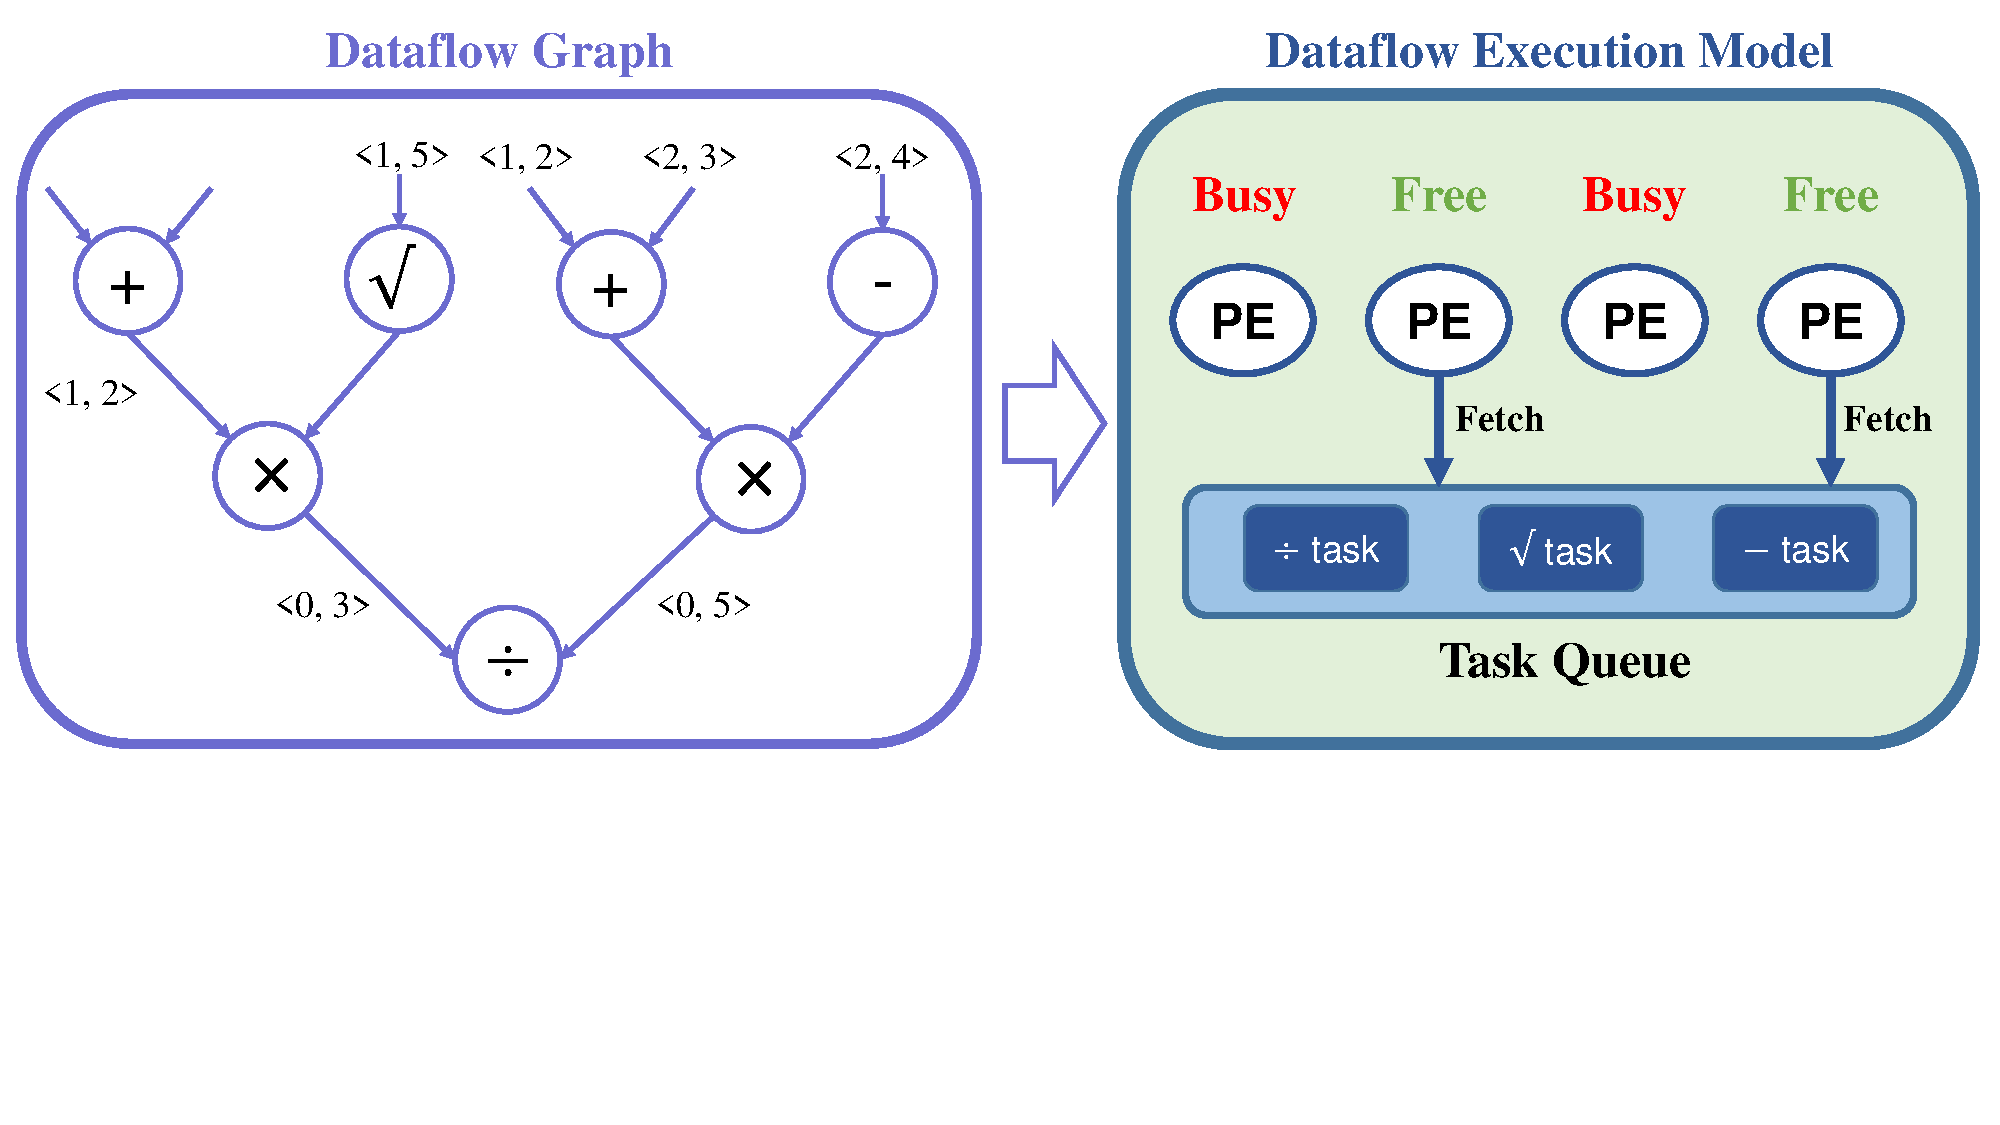
\includegraphics[width=4in]{pics/dataflowModel.pdf}
\vspace{-60pt}
\caption{Dataflow Execution Model}
\label{fig:dataflowModel}
\vspace{-15pt}
\end{figure}

\vspace{-10pt}
\subsection{DCF Dataflow Graph}
%\vspace{-10pt}
In order to design dataflow based gradient descent algorithm, we need to transform the algorithm into dataflow graph expression. As shown in Figure \ref{fig:gdGraph}, we construct dataflow graph of gradient descent according to Eq. \ref{eq:gd1} and Eq. \ref{eq:gd2}. Node $R$ transforms the input data into the triplet form $<user id, item id , rating>$, and sends user id and item id information to $InitU$ and $InitV$ for initializing feature vectors.
%In addition, triplet $<user id, item id, rating>$ is transformed into the key-value pair format $<user id, <item id, rating>>$ and $<item id, <user id, rating>>$.
Meanwhile, node $R$ sends rating data to $U_i$ and $V_i$ for gradient computing, where $U_i$ and $V_i$ represent the $i$th iteration of user node and item node. After initializing feature vectors, $InitU$ and $InitV$ send feature vectors to $U_1$ and $V_1$. In each iteration $i$, $U_i$ and $V_i$ are used to compute the gradients and update feature vectors until convergence. After the gradient computing tasks are finished in last iteration $n$ , $U_n$ and $V_n$ output the trained feature vectors.

\vspace{-10pt}

\begin{figure}[h]
\begin{minipage}[t]{0.45\linewidth}
\centering
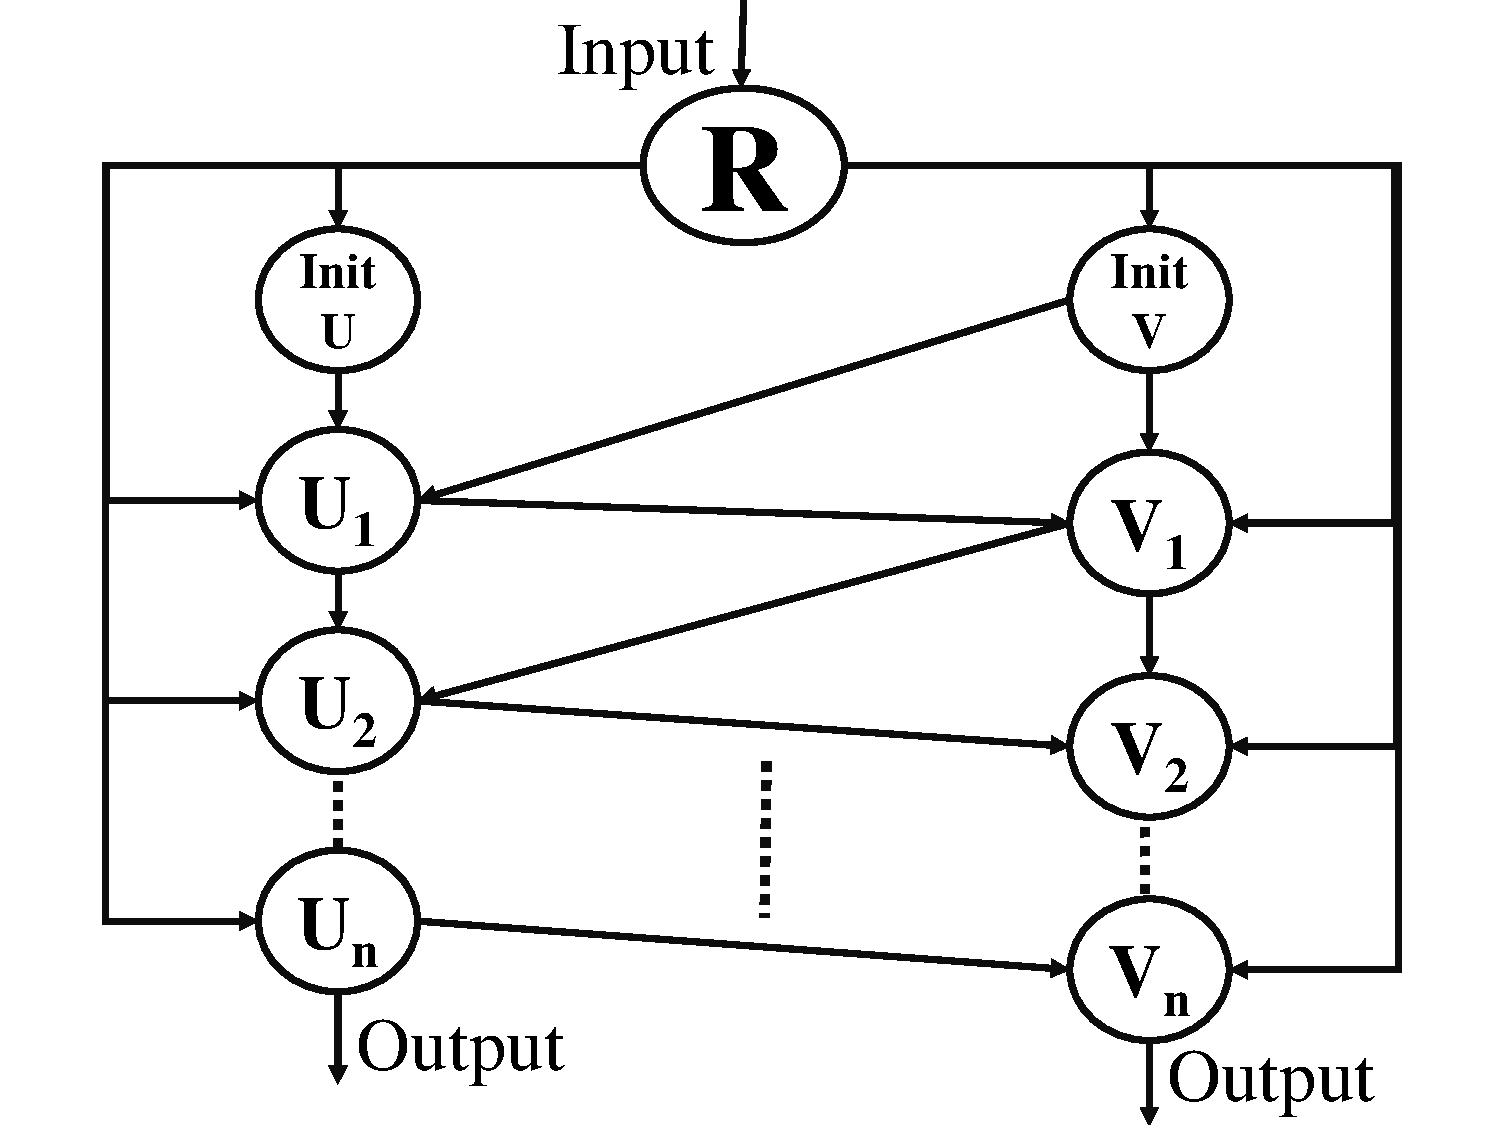
\includegraphics[width=\textwidth]{pics/gdGraph.pdf}
\caption{Dataflow Graph of Gradient Descent \label{fig:gdGraph}}
\end{minipage}
\hfill
\begin{minipage}[t]{0.45\linewidth}
\centering
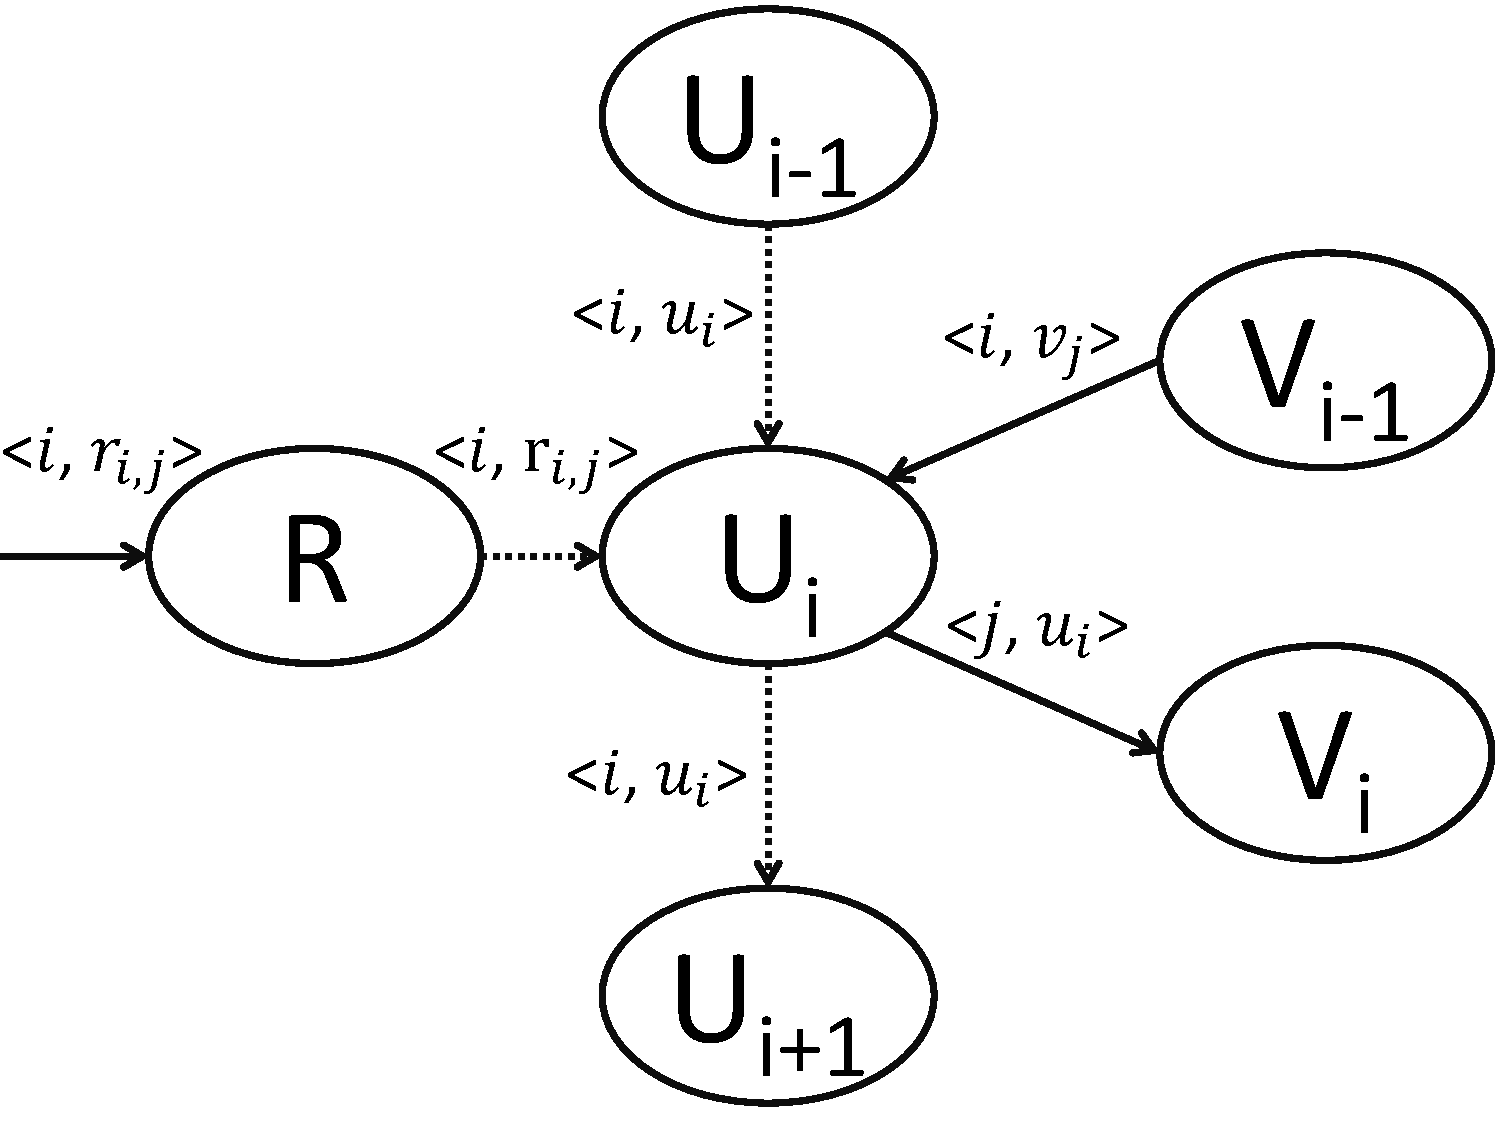
\includegraphics[width=\textwidth]{pics/dummyEdge.pdf}
\caption{Dummy Edge of User Node \label{fig:dummyEdge}}
\end{minipage}
\vspace{-20pt}
\end{figure}

By using dataflow model to implement gradient descent, data sparsity and fine-grain operations can be easily handled. The updating task of each feature vector is scheduled and executed individually. Fine-grain feature naturally supports the updating operation of gradient descent. In addition, the computation load of each feature vector varies in large scale because of the sparse data dependency. Asynchronization feature avoids unnecessary barrier time for waiting hot spot feature vectors in one iteration. As a result, computing resources can be utilized better.

Due to deterministic feature of dataflow model, DCF transform original gradient descent algorithm into dataflow graph without changing the algorithm logic. Hence, DCF shows the same convergency performance with other gradient descent algorithms. Though dataflow model supports gradient descent well, high communication complexity and dependency checking overhead are still challenges can not be solved. Hence, we propose three optimizations to solve these challenges.

\vspace{-10pt}
\subsection{Optimizations}
\subsubsection{Dummy Edge}

We propose dummy edge technique (dashed line in the dataflow graph) to avoid fine-grain overhead of dependency checking and reduce local data movements. As shown in Figure \ref{fig:dummyEdge}, we take the user node $U_i$ as an example to explain dummy edge. The data transferred by dummy edge can be accessed locally because the key of the data does not change. As local data are always ready to be accessed, dependency checking of dummy edge can be avoided.

The reconstructed dataflow graph with dummy edge is shown in Figure \ref{fig:DDCF}. Similar with $R$ in Figure \ref{fig:gdGraph}, $R_U$ and $R_V$ transforming rating data into triplet format, are indexed by user id and item id respectively, in order to be locally accessed by $U$ and $V$. As for gradient computing nodes $U$ and $V$, two input edges are replaced by two dummy edges , and the other input edge remains unchanged. Data movements can be reduced because only feature vectors from normal edge
%(user feature vectors from $U$ to $V$, item feature vectors from $V$ to $U$)
should be transferred by network.
%The dependency checking overhead can also be reduced because there is no.
There is no dependency checking operation of every node in reconstructed dataflow graph because there is only one normal input edge of them.
\vspace{-10pt}

\begin{figure}[h]
\begin{minipage}[t]{0.45\linewidth}
\centering
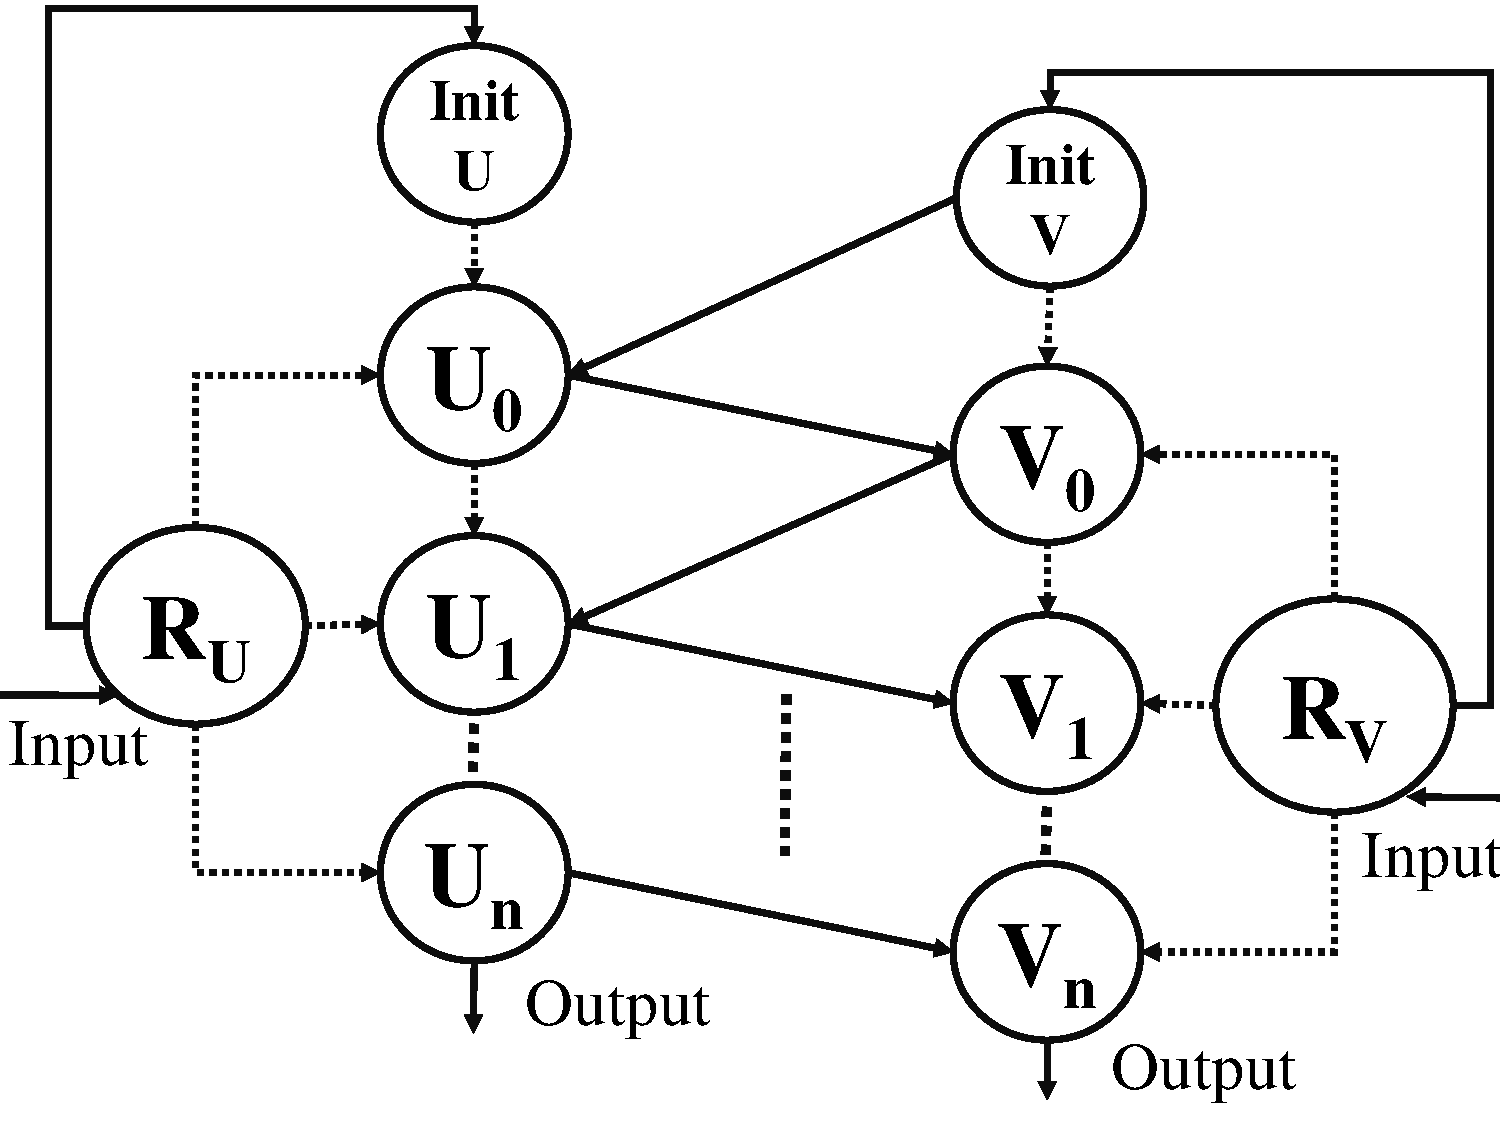
\includegraphics[width=\textwidth]{pics/DDCF.pdf}
\caption{Dataflow Graph of Gradient Descent Using Dummy Edge \label{fig:DDCF}}
\end{minipage}
\hfill
\begin{minipage}[t]{0.5\linewidth}
\centering
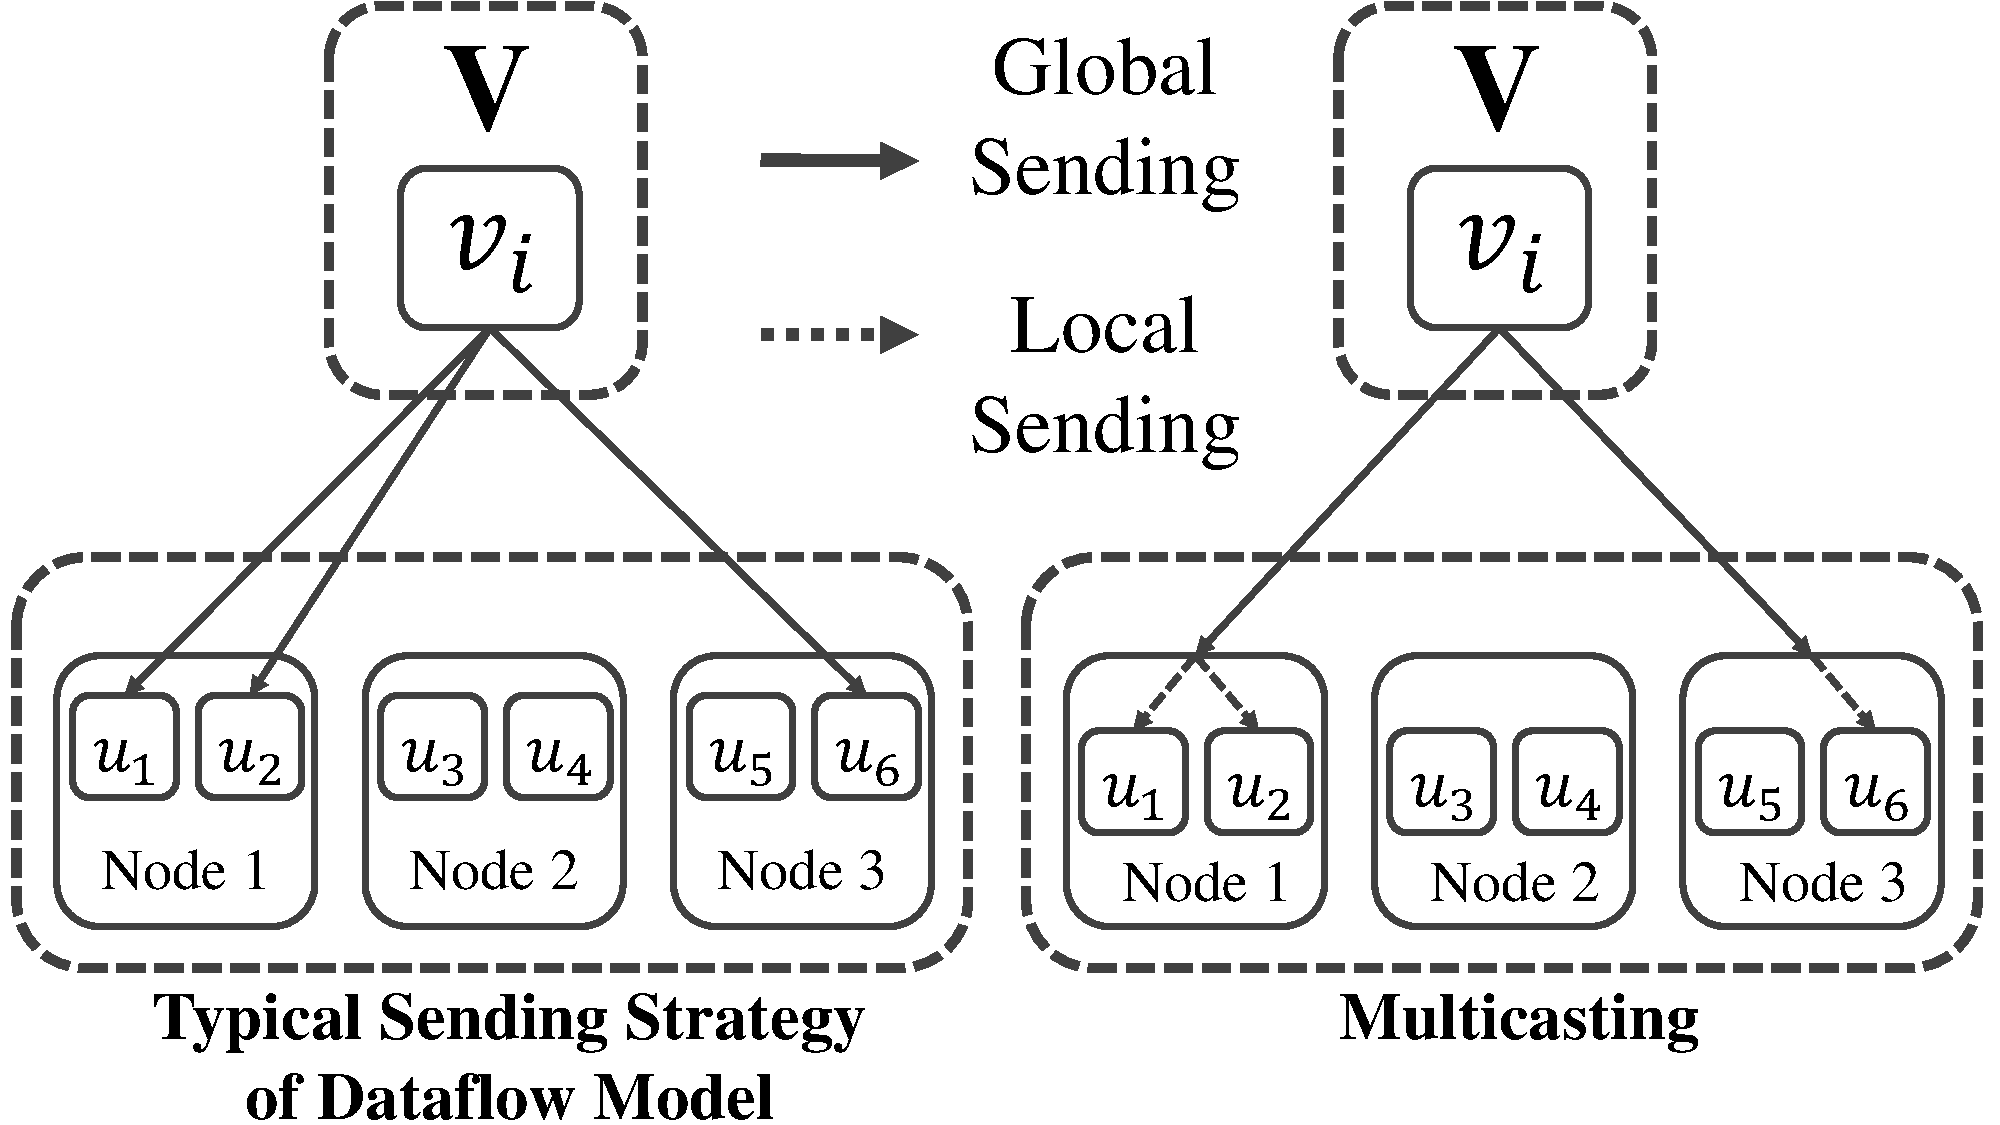
\includegraphics[width=\textwidth]{pics/multicasting.pdf}
\caption{Sending Strategy of Naive Dataflow Model \label{fig:multicasting}}
\end{minipage}
\vspace{-20pt}
\end{figure}

%In summary, dummy edge can effectively remove the fine-grain overhead of dependency checking. It can also reduce unnecessary data movements of ratings and feature vectors.
\vspace{-15pt}
\subsubsection{Multicasting}
With dummy edge, data movements can be reduced by avoiding sending local data. However, the quantity of data transferred by normal edges is much more than that by two dummy edges. Hence, we propose multicasting strategy to further optimize the data movements. As shown in Figure \ref{fig:multicasting}, global sending means sending data to different nodes in the cluster through network, while local sending means sending data in the node without network. In the scenario of sending data from $V$ to $U$, typical sending strategy of dataflow model requires data to be sent to the location of dependent users by global sending directly. In this process, key-value pairs with the same value may be sent to different locations on the same node. For example, the key-value pairs sent to $u_1$ and $u_2$ on node 1 has the same value $v_i$. Repetitive data sent to the same node will increase the network load of the algorithm. As for multicasting strategy, key-value pairs of same feature vectors are sent to the nodes which have dependent feature vectors by global sending. For example, $v_i$ depends on user $u_1$, $u_2$ and $u_6$, and there is no dependent data on node 2. Key-value pairs of $v_i$ are sent to node 1 and 3 first by global sending. Then, each node sends the key-value pairs to dependent feature vectors by local sending. $u_1$ and $u_2$ get the key-value pair from node 1 and $u_6$ gets the key-value pair from node 3.

Compared with original the communication complexity described in Section \ref{sub:gd}, the complexity by using multicasting is $O(ck(n_u + n_v))$ where $c$ represents the node number of cluster. The complexity is reduced by $\bar{d}/c$ times where average dependency number $\bar{d}$ increases with rating data linearly. In conclusion, multicasting can significantly reduce data movements in large scale dataset.
\vspace{-15pt}
\subsubsection{Mini-batch}

Mini-batch \cite{Dean2012} was firstly proposed to improve the performance by limiting batch size of each iteration in deep learning scenarios . Hence, we apply mini-batch technique in collaborative filter for reducing computation and communication complexities. While the batch size of each feature vector is different in collaborative filtering, we select the minimal number between dependency number $d$ and mini-batch size $b$ as the final dependency number for each feature vector. In large rating scenario, the mini-batch $b$ is always set as the final dependency number because real dependency number $d$ is larger than mini-batch size $b$. The computation and communication complexities of one iteration are $O(kb(n_u + n_v))$, and the complexities are reduced by $\bar{d}/b$ times where average dependency number $\bar{d}$ increases with rating number linearly. As a result, mini-batch technique can significantly reduce the computation and communication in large scale datasets.

We evaluate all optimizations in Section \ref{sub:opt} and the experiments results shows that these optimizations can significantly improve the performance of our algorithm.

\vspace{-15pt}
\subsection{DCF Algorithm}
\vspace{-5pt}
By Applying dummy edge, multicasting and mini-batch optimizations, we get the finalized algorithm. In order to design a dataflow based algorithm, we need to construct a dataflow graph and give detailed algorithms for each node in the graph. The finalized dataflow graph is shown in Figure \ref{fig:DDCF}. The key nodes are gradient computing nodes ($U$ and $V$), while other nodes are used to preprocess data. As the algorithm logic is same for $U$ and $V$, we give the detailed algorithm of user node $U$.

%\vspace{-10pt}
\begin{algorithm}
\caption{Execution Process of DCF User Node $U$}
\label{code:DCF}
\begin{algorithmic}[1]
\STATE Receive $<i, v_j>$ from upstream node
\STATE Get $u_i$ from user data, get $r_{i,j}$ from rating data
\IF {$d_{u_i}$ for $u_i$ is not initialized}
\STATE Get $n_{u_i}$ from rating data
\STATE $d_{u_i} = min(b,n_{u_i})$
\STATE $u_{sum} = 0$
\ENDIF
\IF {$d_{v_j}$ for $v_j$ is not initialized}
\STATE $d_{v_j} = b$
\ENDIF
\IF {$d_{u_i} > 0$}
\STATE Get $r_{i,j}$ from rating data
\STATE $u_{sum} = u_{sum} + (u_i^T v_j - r_{i,j})v_j$
\STATE $d_{u_i} = d_{u_i} - 1$
\ENDIF
\IF {$d_{u_i} = 0$}
\STATE $u_i = u_i - \alpha (u_{sum} + \lambda u_i)$
\FOR {all $v_k$ of $u_i$}
\IF {$d_{v_k} > 0$}
\STATE Send $<k, u_i>$ to dependent $v_k$ using multicasting
\STATE $d_{v_k} = d_{v_k} - 1$
\ENDIF
\ENDFOR
\ENDIF
\end{algorithmic}
\end{algorithm}


According to dummy edge technique, user vector $u_i$ and rating $r_{i,j}$ are obtained by querying with user id $i$ and item id $j$ after receiving the key-value pair $<i, v_j>$ in lines 1-2. In lines 3-6, temporary gradient $u_{sum}$ and dependency counter $d_{u_i}$ are initialized to record the intermediate result of gradient computing, instead of checking redundant dependency. In line 5 and 7-8, mini-batch strategy is applied to initialize the dependency counter $d_{u_i}$ and the sending counter $d_{v_j}$ for reducing computation and communication complexities. If $d_{u_i} > 0$, gradient will be added to the temporary gradient $u_{sum}$ in lines 9-12. In lines 13-18, if the item dependencies for $u_i$ are satisfied ($d_{u_i} = 0$) and ), $u_i$ will be updated by temporary gradient $u_{sum}$ and old feature vector $u_i$. For every dependent items $v_k$ of $u_i$, if the sending dependency is satisfied ($d_{v_k} > 0$), the updated $u_i$ will be sent to the item $v_k$ by multicasting.
%\vspace{-30pt}
%
\vspace{-10pt}
\section{Experiments}
\label{sec:experiment}
\vspace{-5pt}
%\subsection{Experimental Setup}

% TODO: ʵÏְ江µÄÄÚÈÝžùŸÝÒÑÓеÄʵÑéÊýŸÝµ÷Õû
% žÅÀÀ£¬×ÜœáʵÑ鲿·Ö¶Ô±ÈÄÚÈÝ£¬ºáÏò¶àƜ̚¶Ô±È£¬×ÝÏòÓÅ»¯¶Ô±È£¬ÍØÕ¹ÐÔʵÑé

We implement DCF with Java and evaluate its performance on public datasets under both multicore and distributed platforms. Spark ALS \cite{SparkMllib} and Graphlab \cite{graphlab} gradient descent (Graphlab GD) are two most widely used distributed collaborative filtering algorithms, so we select them as the contrasts of DCF. We evaluate the performance of optimizations (dummy edge, multicasting and mini-batch) separately. Scalability of DCF over contrast algorithm are assessed at the last of this section. In all the experiments, we use 1 master + 10 slaves cluster. The CPU of each node is Intel(R) Xeon(R) E5-2630 with 32 cores and the memory of each node is 128G. As for parameter setting, default iteration is 10 and mini-batch size is 40.
%\vspace{-15pt}

%\begin{table}[!htb]
%\renewcommand{\arraystretch}{1.3}
%\caption{Configuration of Experiment Machine}
%\label{tab:cluster}
%\centering
%\begin{tabular}{|c|c|c|c|}
%\hline
%Operating System & CPU & Core Number & Memory\\
%\hline
%CentOS 6.7 & Intel(R) Xeon(R) E5-2630 & 32 & 128G\\
%\hline
%\end{tabular}
%\vspace{-15pt}
%\end{table}

Movielens, Netflix and Yahoo Music are the three datasets used in the experiments. Detailed information of the datasets are shown in Table \ref{tab:dataset}. We use 80\% data for training and 20\% data for testing in each dataset.

\vspace{-10pt}
\begin{table}[!htb]
\renewcommand{\arraystretch}{1.3}
\caption{The Statistical Information of Each Dataset}
\label{tab:dataset}
\centering
%\begin{tabular}{|c{2cm}|p{2cm}|p{2cm}|p{2cm}|}
\begin{tabular}{|c|c|c|c|}
\hline
\textbf{Dataset} & Movielens & Netflix & Yahoo Music\\
\hline
user number & 260,000 & 480,190 & 1,000,990\\
\hline
item number & 40,000 & 17,770 & 624,961\\
\hline
rating & 24,000,000 & 99,072,112 & 252,800,275\\
\hline
\end{tabular}
\vspace{-30pt}
\end{table}

\subsection{Comparing DCF with Other Distributed Algorithms}
\label{sub:dcf}

\textbf{Performance:} Figure \ref{fig:dcfPerformance} shows the results of DCF comparing with Spark ALS and Graphlab GD under public datasets. The trends of three algorithms are the same under different datasets. DCF shows the best performance among three algorithms. The speedup of DCF over Graphlab ranges from 5.4 to 18.01 and the average speedup is 9.76. Compared with Graphlab GD, the results demonstrate that DCF significantly improves the performance of gradient descent on distributed platform by applying dataflow with optimizations. The speedup of DCF over ALS ranges from 1.15 to 23.01 and the average speedup is 4.6. As $k$ increases, the training time increases linearly with DCF but quadratically with ALS. When $k=400$, DCF can achieve 14.34 speedup over ALS on average. The results prove the computation complexity analysis in Section \ref{sec:background}, and show that DCF outperforms ALS due to algorithm selection and the design.

As rating size is different in three datasets, DCF shows better performance with increasing rating size. In Movielens, Netflix and Yahoo Music, DCF has an average speedup of 3.0, 3.9, 6.9 over ALS, and 5.81, 8.29, 15.11 over Graphlab GD. In three datasets, movielens has the smallest ratings and Yahoo Music has the largest ratings. DCF shows the best performance in the largest dataset.

\begin{figure}[!t]
\centering
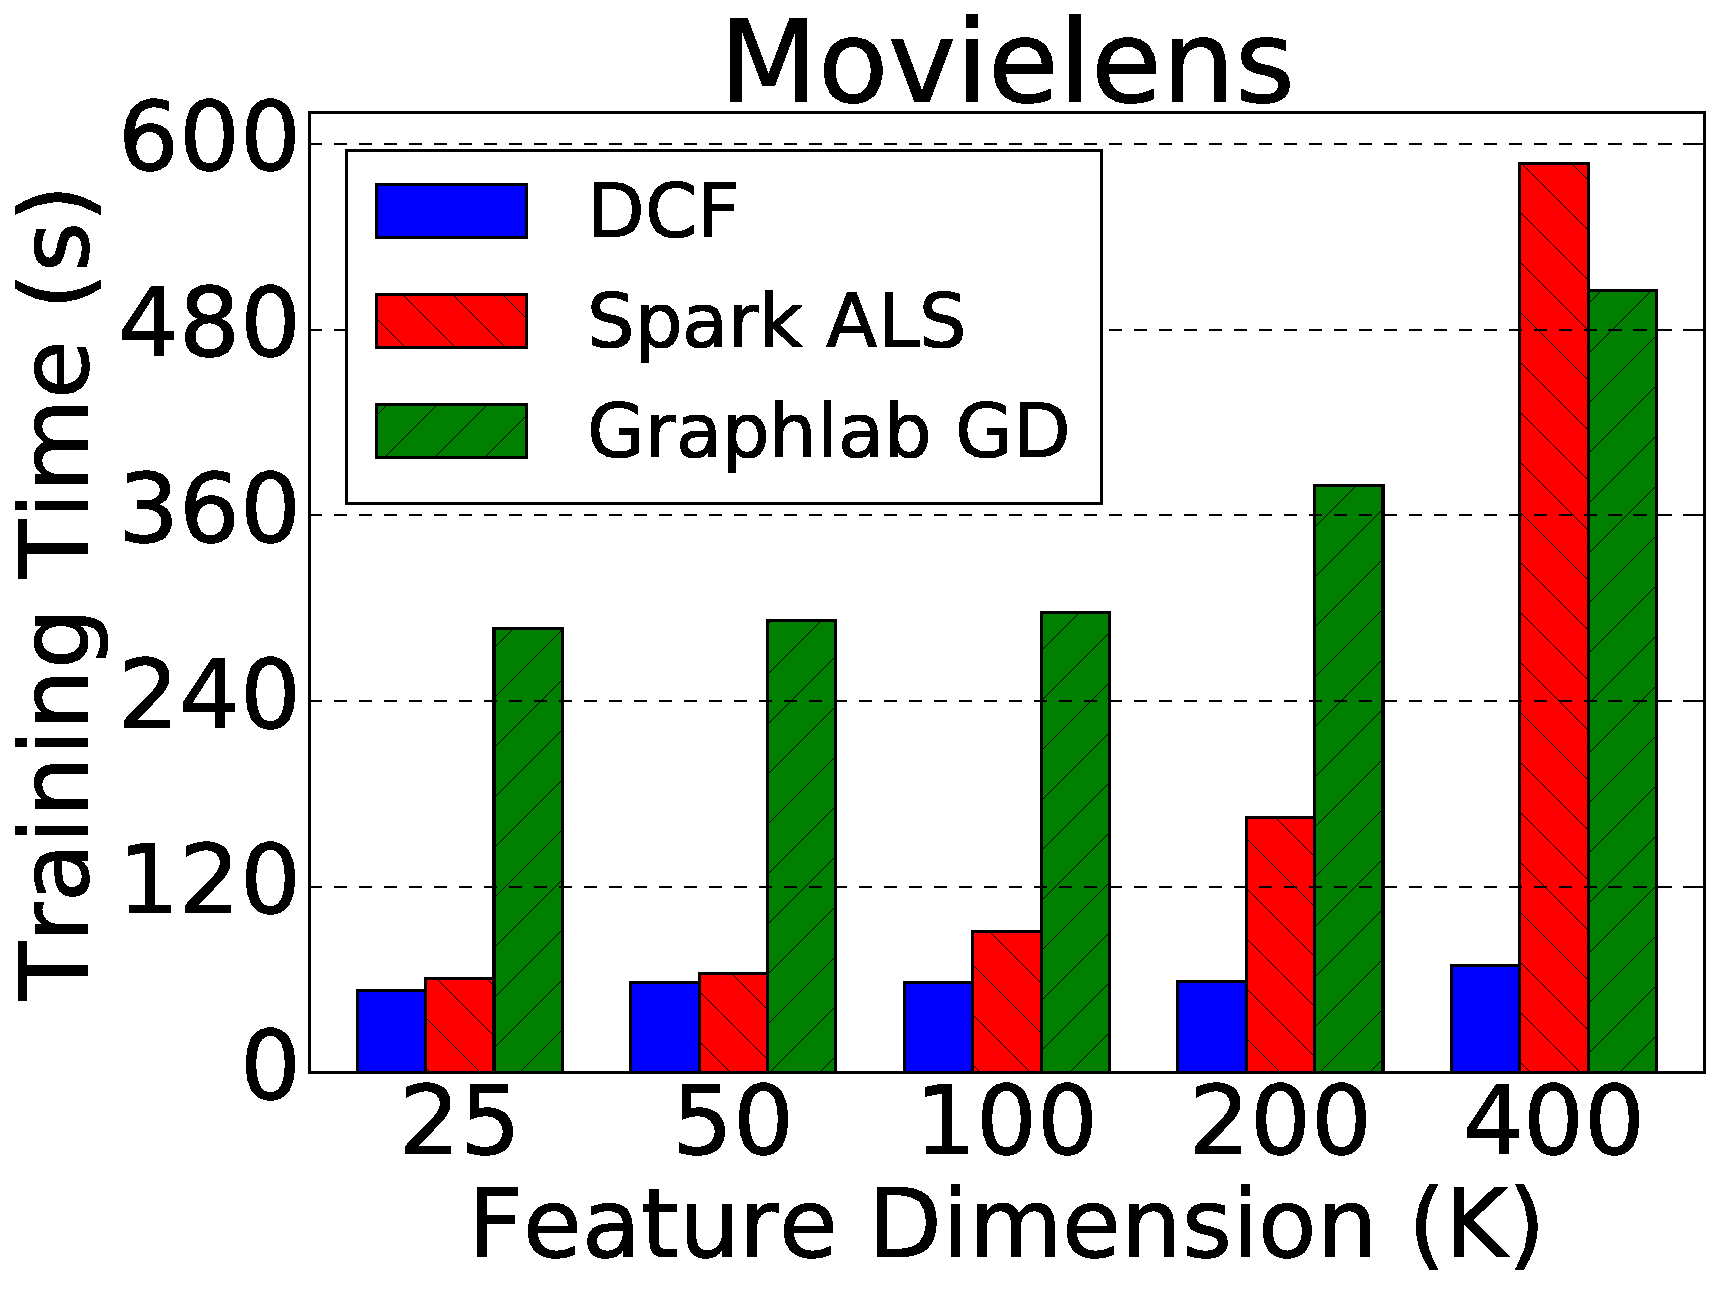
\includegraphics[width=1.5in]{pics/movielens.pdf}
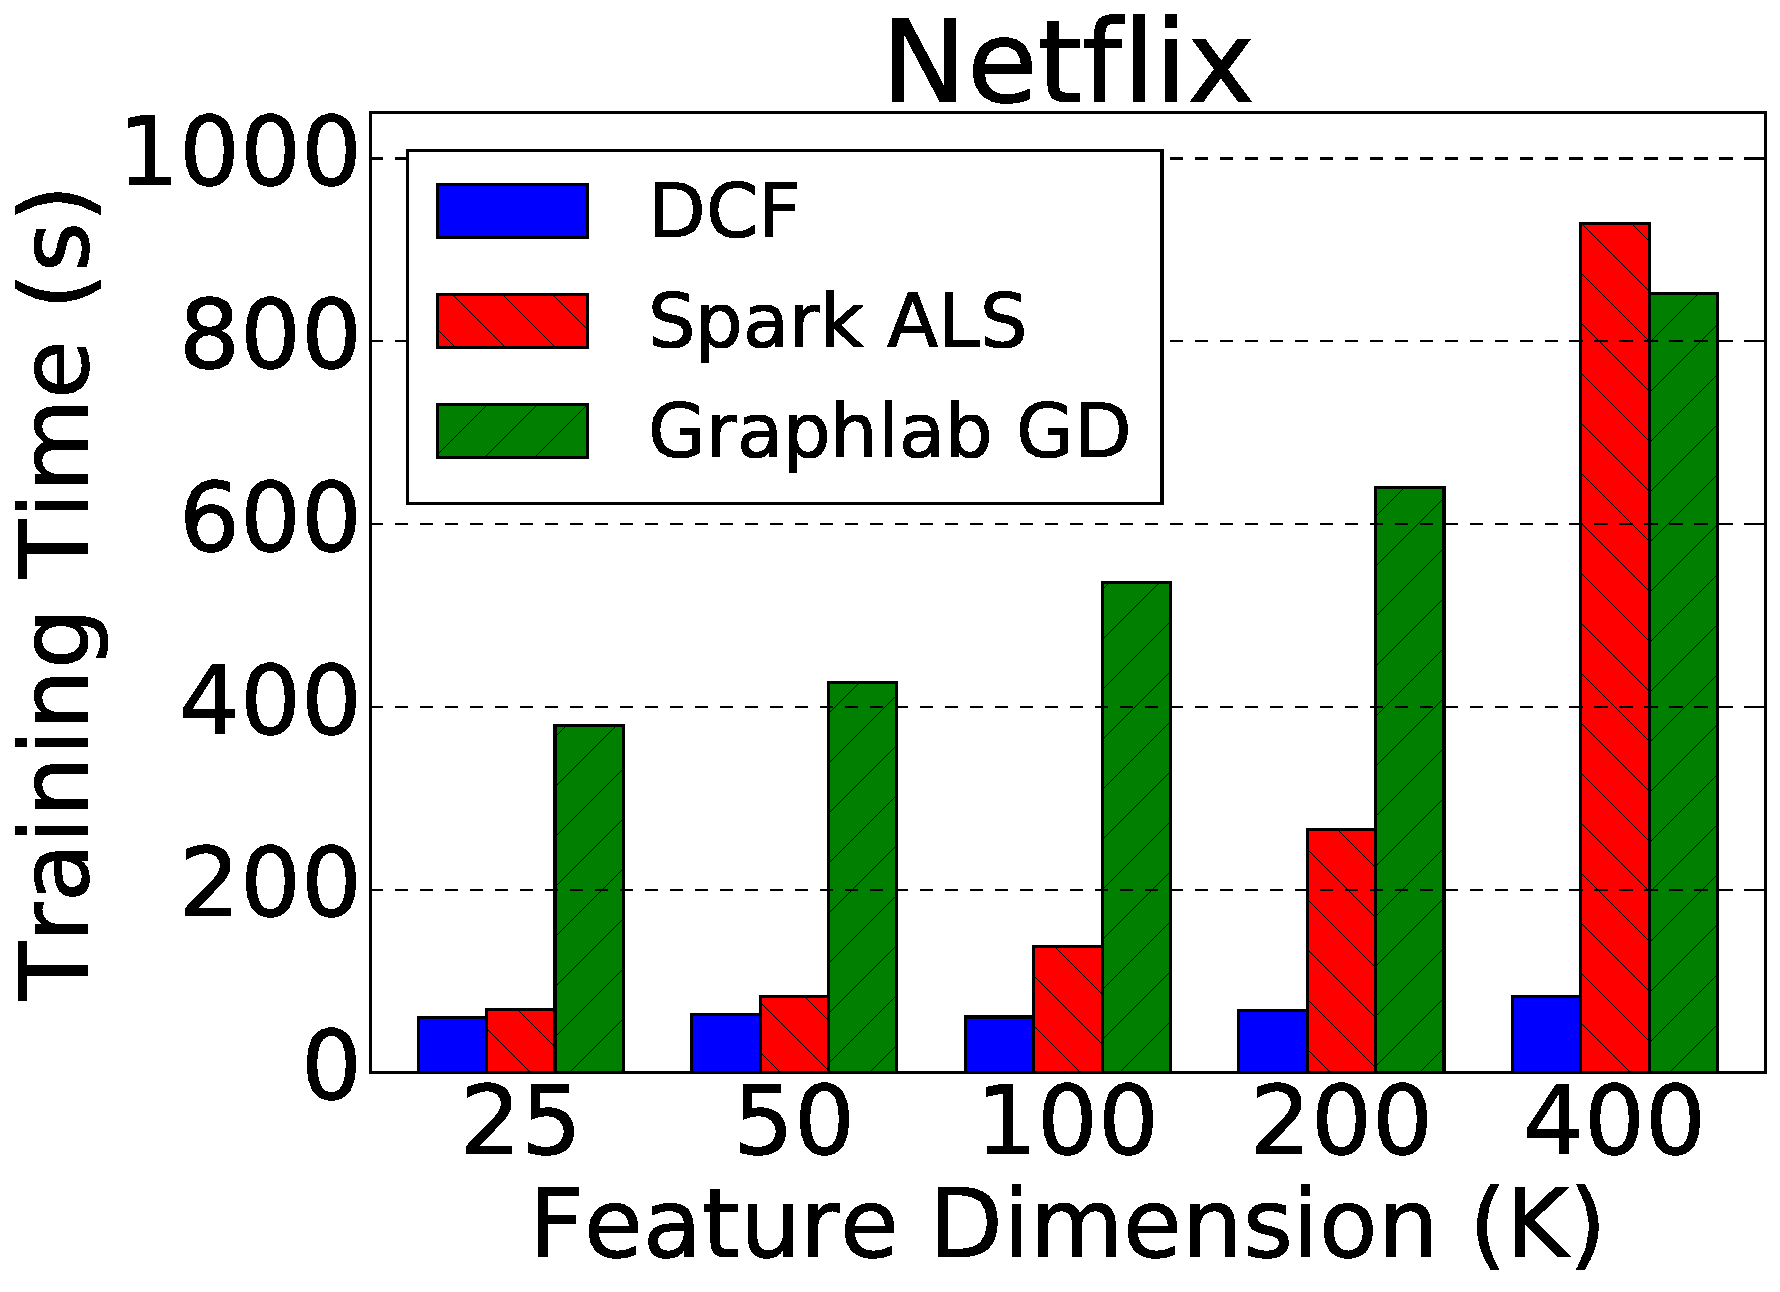
\includegraphics[width=1.5in]{pics/netflix.pdf}
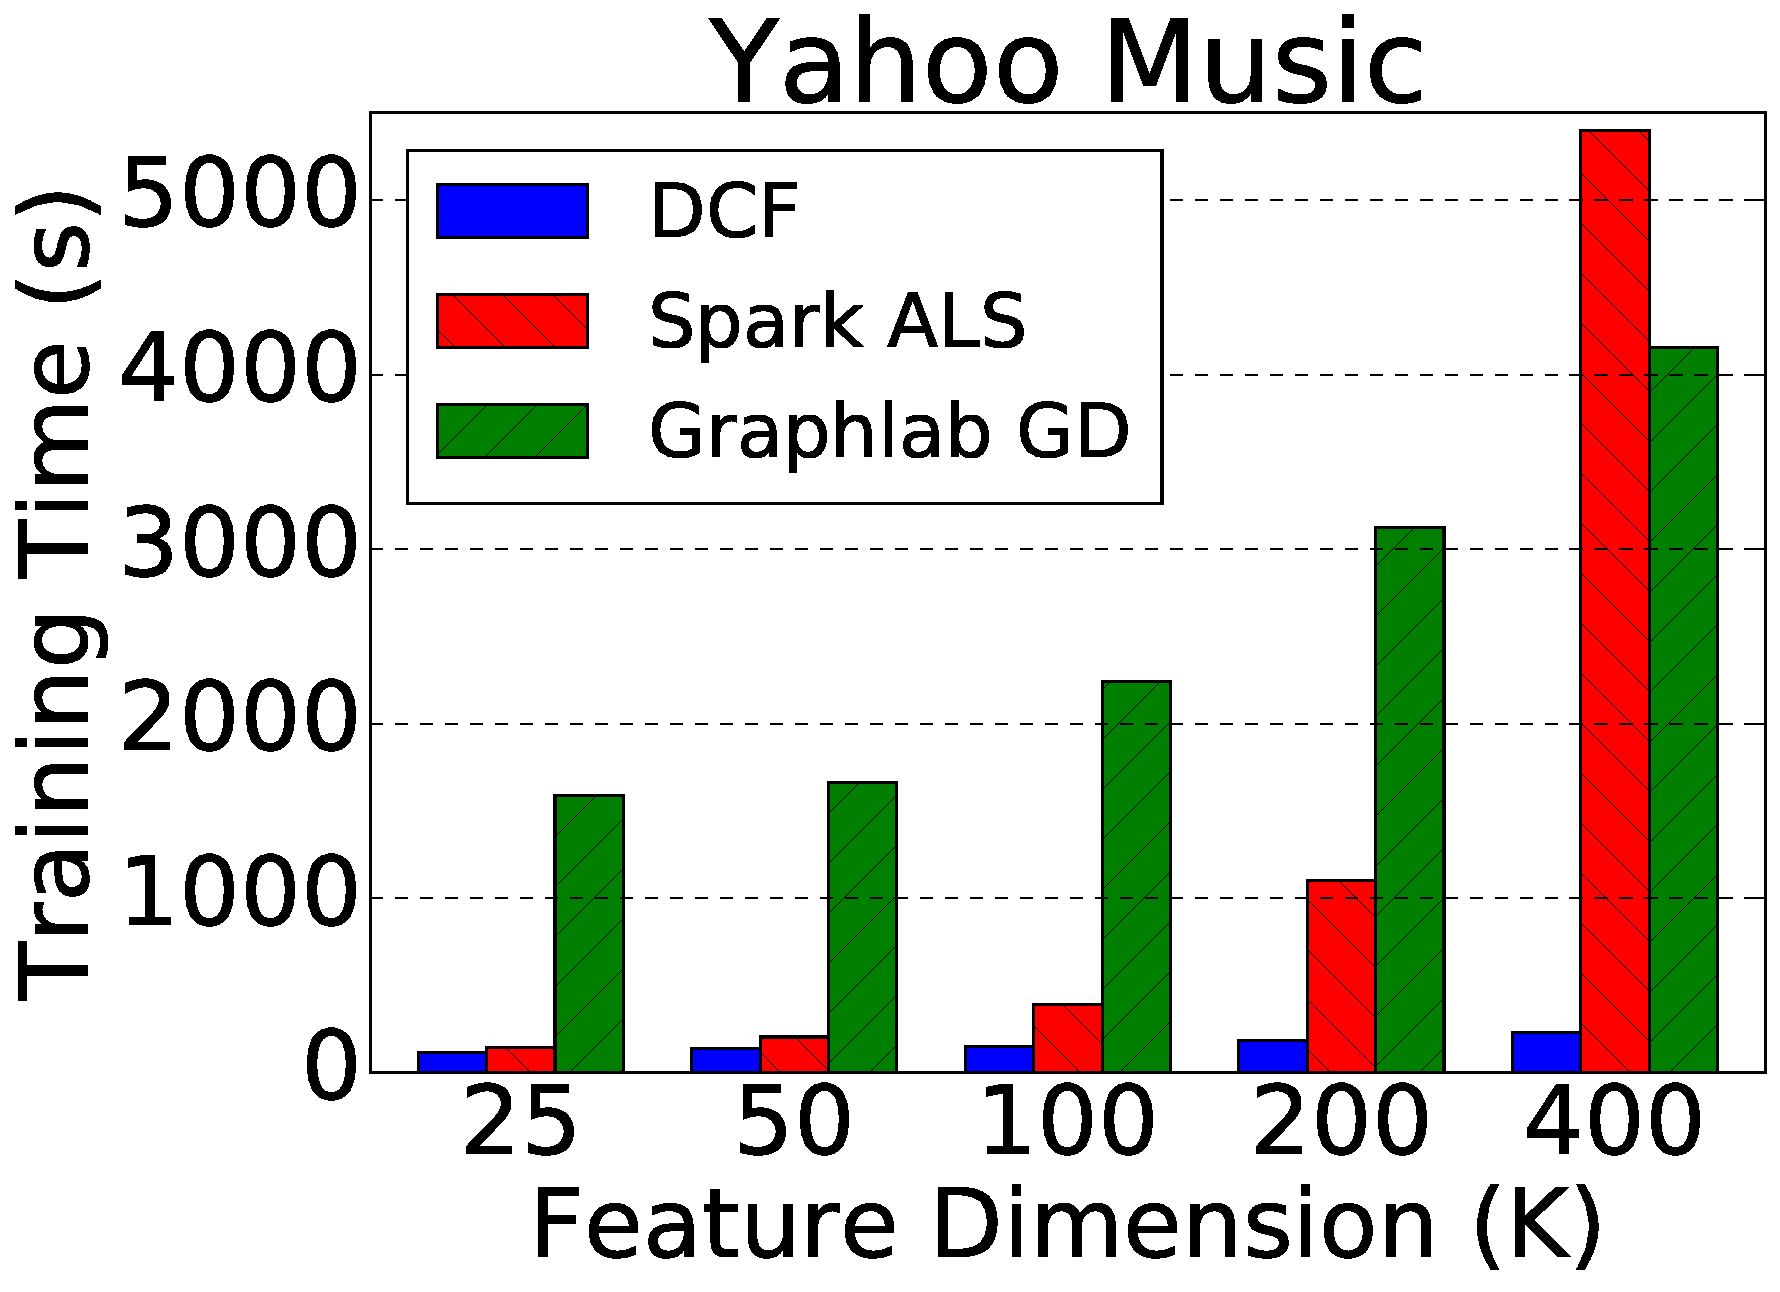
\includegraphics[width=1.5in]{pics/yahoo.pdf}
\caption{Comparisons of DCF With Other Distributed Algorithms Under Public Datasets}
%\centering
\vspace{-15pt}
\label{fig:dcfPerformance}
\end{figure}

\textbf{Accuracy:} We also evaluate the accuracy of three algorithms on Netflix dataset. Root mean square error (RMSE) \cite{towards} is the general metrics for model based collaborative filtering algorithms. With smaller RMSE, the algorithms show better convergency performance. To get RMSE at 0.95, DCF, ALS and Graphlab GD converge with iterations of 9, 6 and 9 respectively. According above data of iteration time, DCF achieves the same accuracy with significantly improvements in performance. In addition, DCF shows the same convergency performance with other distributed gradient descent algorithms.

%\begin{equation}
%\label{eq:rmse}
%  RMSE=\sqrt \frac{{\sum_{r_{i,j}\neq 0}{(r_{i,j}-\hat{r}_{i,j})}^2}}{n}
%\end{equation}

\vspace{-10pt}
\subsection{Optimizations Evaluation}
\vspace{-5pt}
\label{sub:opt}

In this subsection, we evaluate the optimizations of DCF algorithm in Netflix dataset. As shown in left part of Figure \ref{fig:opt}, there are four experiment algorithms used to evaluate dummy edge and multicasting. DCF-Naive represents the algorithm without using proposed optimizations and mini-batch technique is not applied to four experiment algorithms. DCF-Naive with multicasting has a speedup of 2.04 over DCF-Naive. When $k$ increases, it shows better performance, and the speedup goes up to 3.87. The results prove that multicasting can significantly improve the performance by reducing data movements. The speedup of DCF-Naive with dummy edge over DCF-Naive is not distinct. With multicasting, dummy edge can improve the performance by 30\% on average. However, dummy edge improve the performance less than 5\% without multicasting. This difference in two comparisons indicates that data movements is the primary challenge in this algorithm. In conclusion, dummy edge and multicasting can significantly improve the performance.


\begin{figure}[!t]
\centering
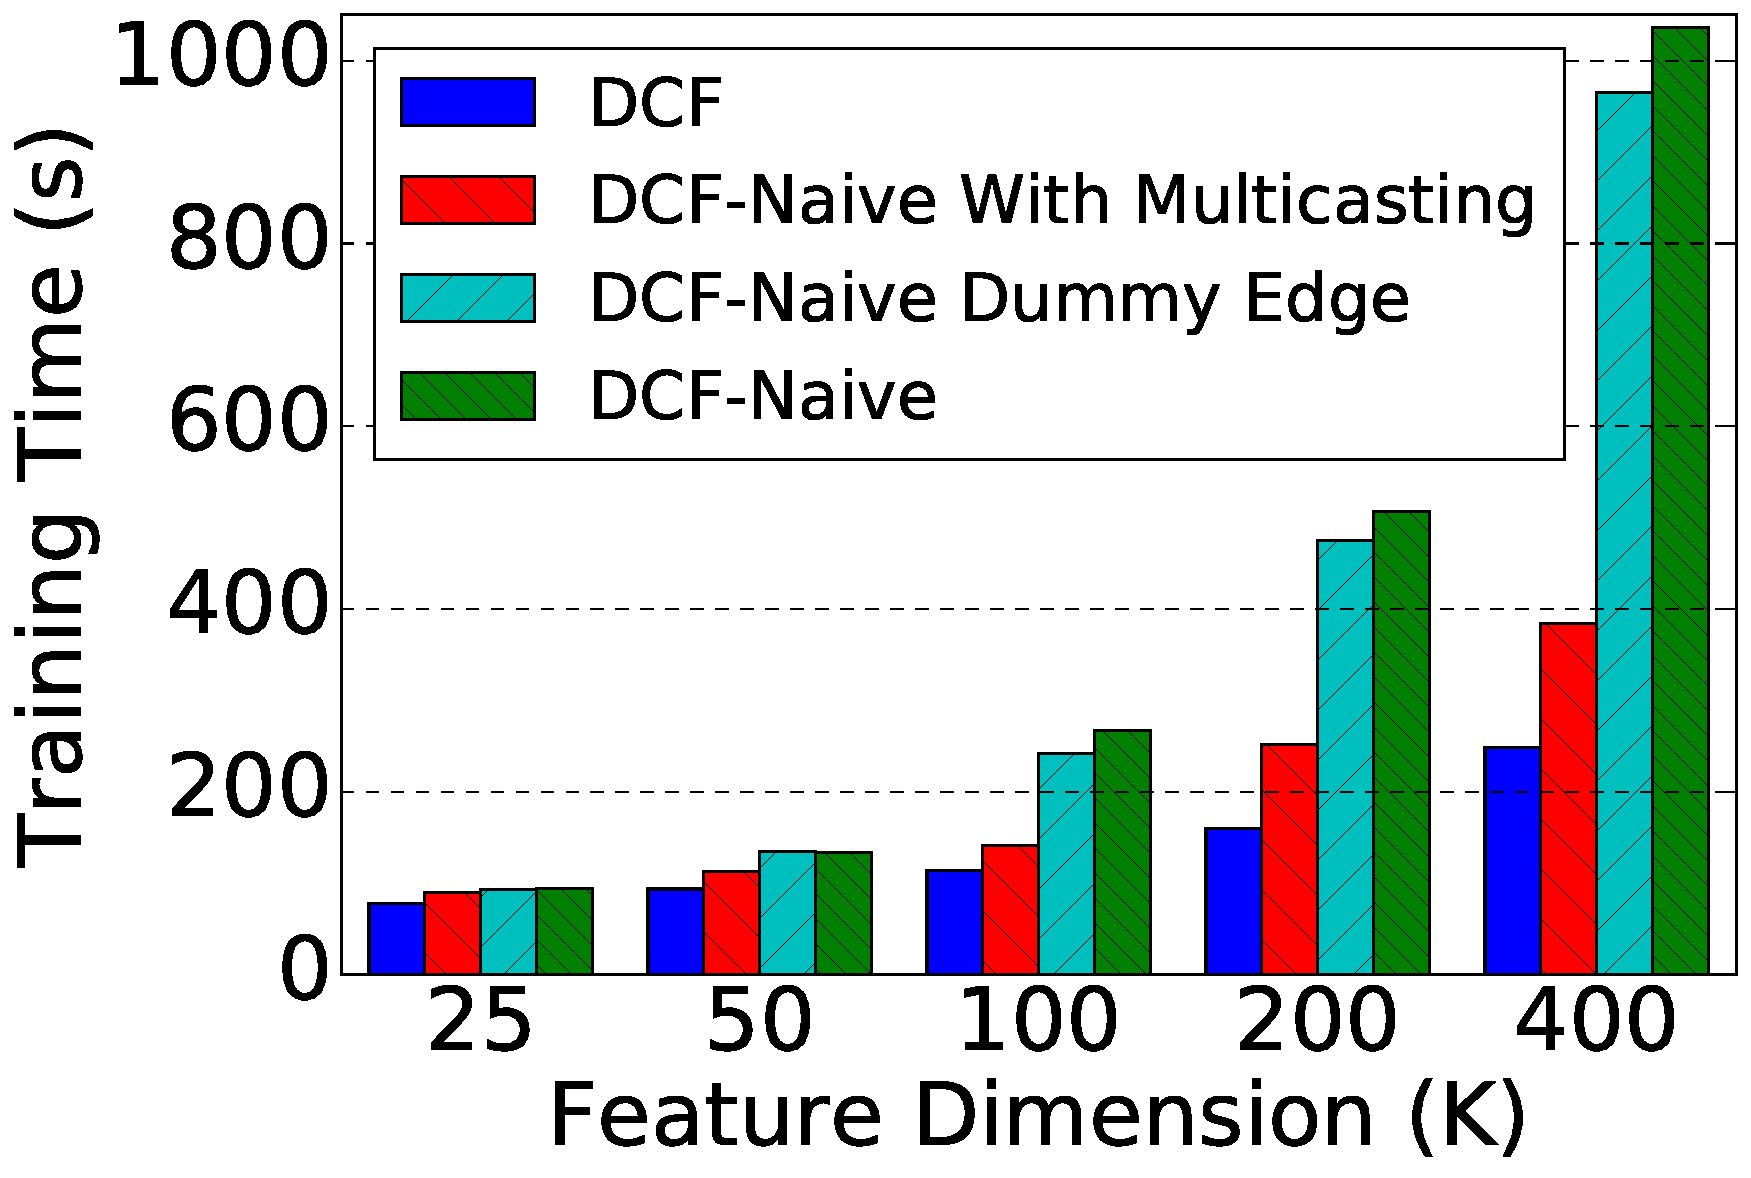
\includegraphics[width=2in]{pics/opt.pdf}
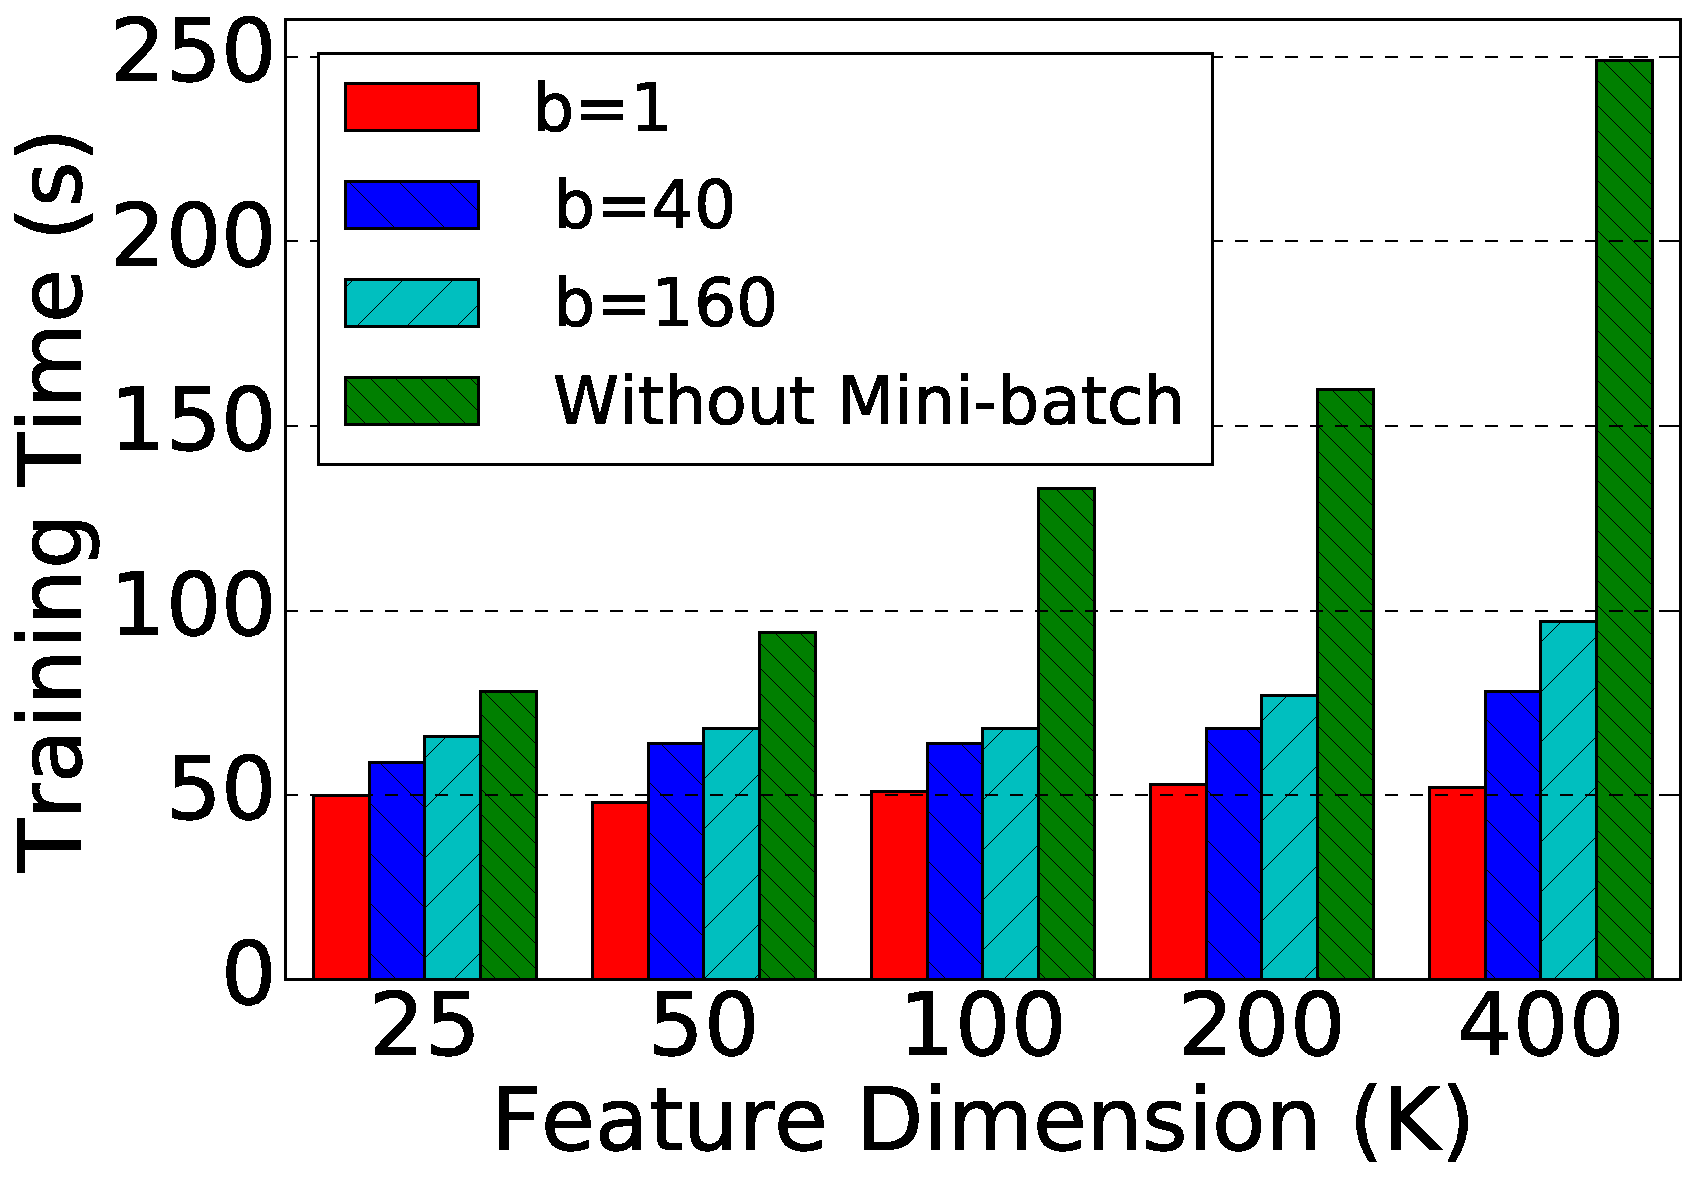
\includegraphics[width=2in]{pics/mb.pdf}
\vspace{-10pt}
\caption{Optimizations Evaluation of DCF}
\label{fig:opt}
\end{figure}

%\begin{figure}[!t]
%\centering
%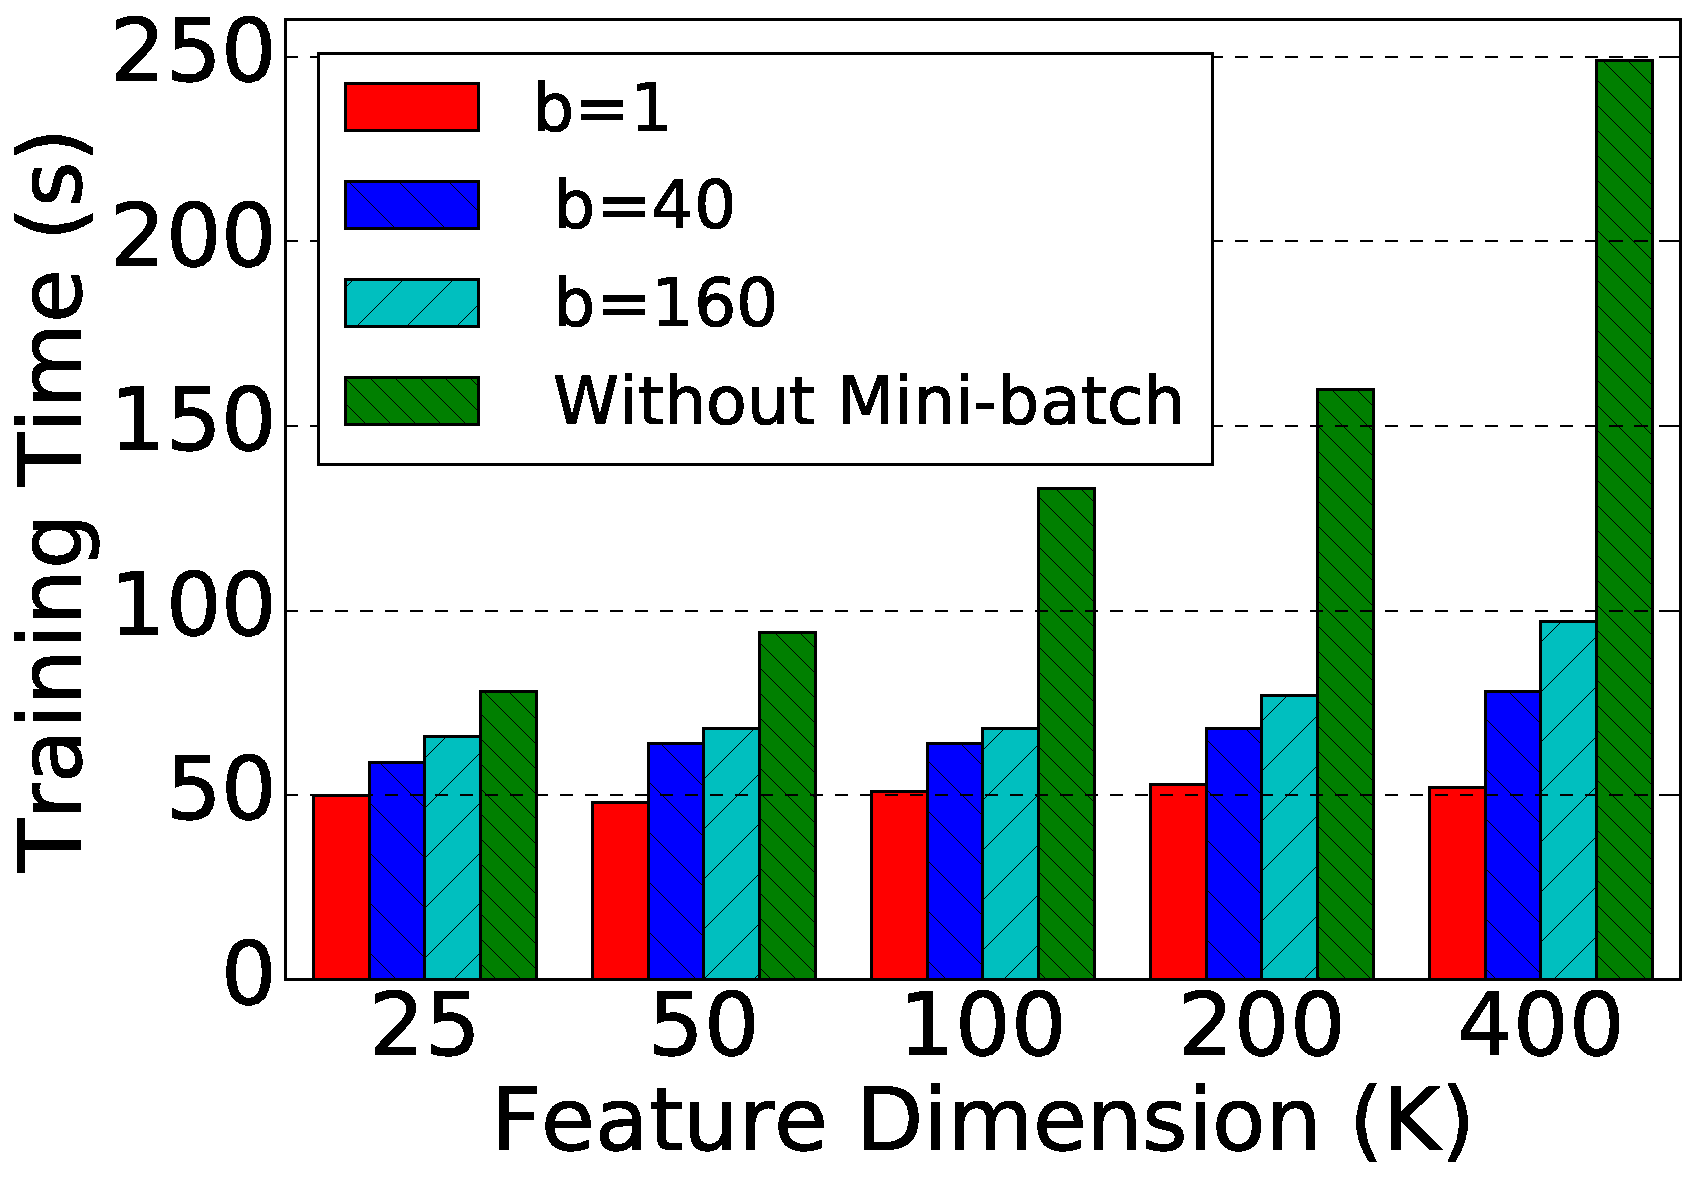
\includegraphics[width=2.5in]{pics/mb.pdf}
%\caption{Mini-Batch Evaluation of DCF}
%\vspace{-10pt}
%\label{fig:mb}
%\end{figure}

As shown in the right part of Figure \ref{fig:opt}, we also evaluate mini-batch technique of DCF. $b = 1$ is a special case to set the dependency number to minimal value. Compared $b=40$ with not using mini-batch situation, the speedup of using mini-batch strategy ranges from 1.32 to 3.19, and the average speedup is 2.08. The results demonstrate that mini-batch technique can improve the performance by optimizing computation and communication complexities. With decreasing $b$, mini-batch technique does not show obvious improvement when $b$ is less than 40. $b=40$ situation takes 31.02\% longer training time than $b=1$, which can be considered as a similar performance with $b=1$. However, the convergence speed of $b=1$ is much lower than other situations. As a result, $b=40$ is the best situation balancing the performance and the convergency.

\begin{figure}[!t]
\centering
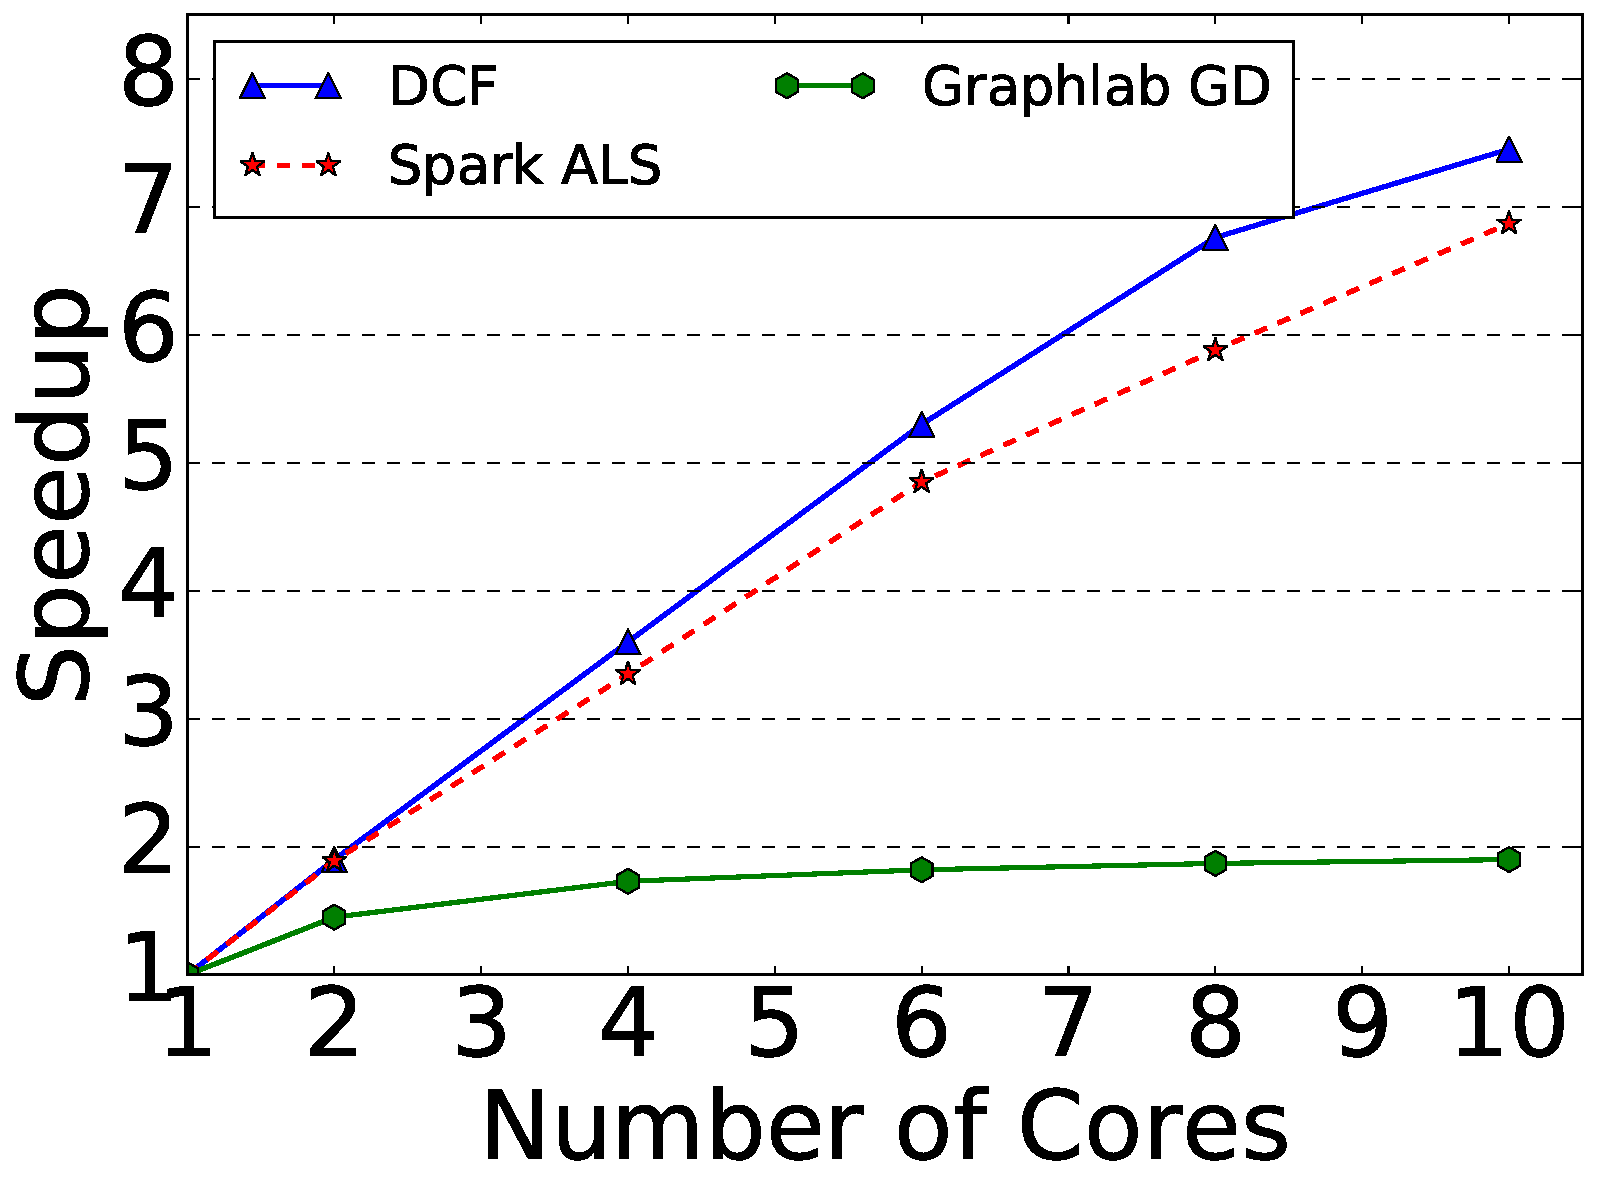
\includegraphics[width=2in]{pics/core.pdf}
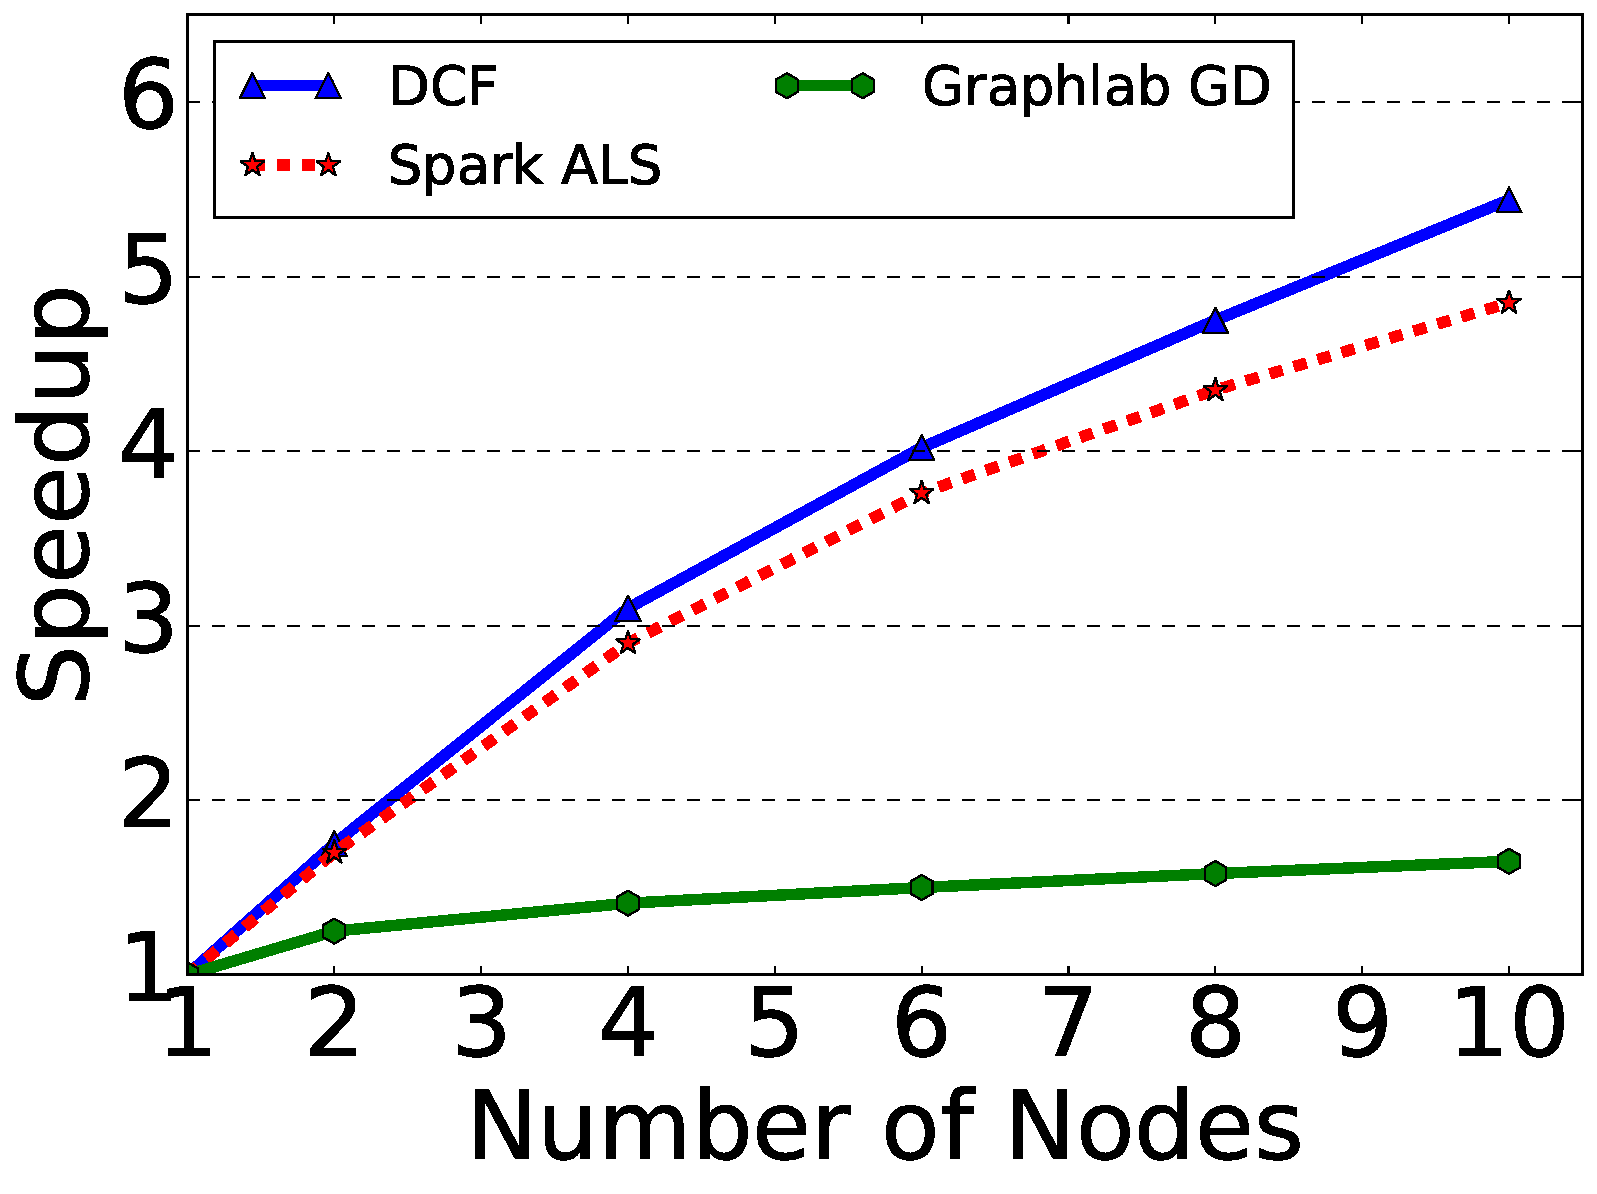
\includegraphics[width=2in]{pics/node.pdf}
\vspace{-10pt}
\caption{Speedup Comparisons of Three Algorithms in Multicore System and Distributed System}
\vspace{-15pt}
\label{fig:core}
\end{figure}


%\begin{figure}[!t]
%\centering
%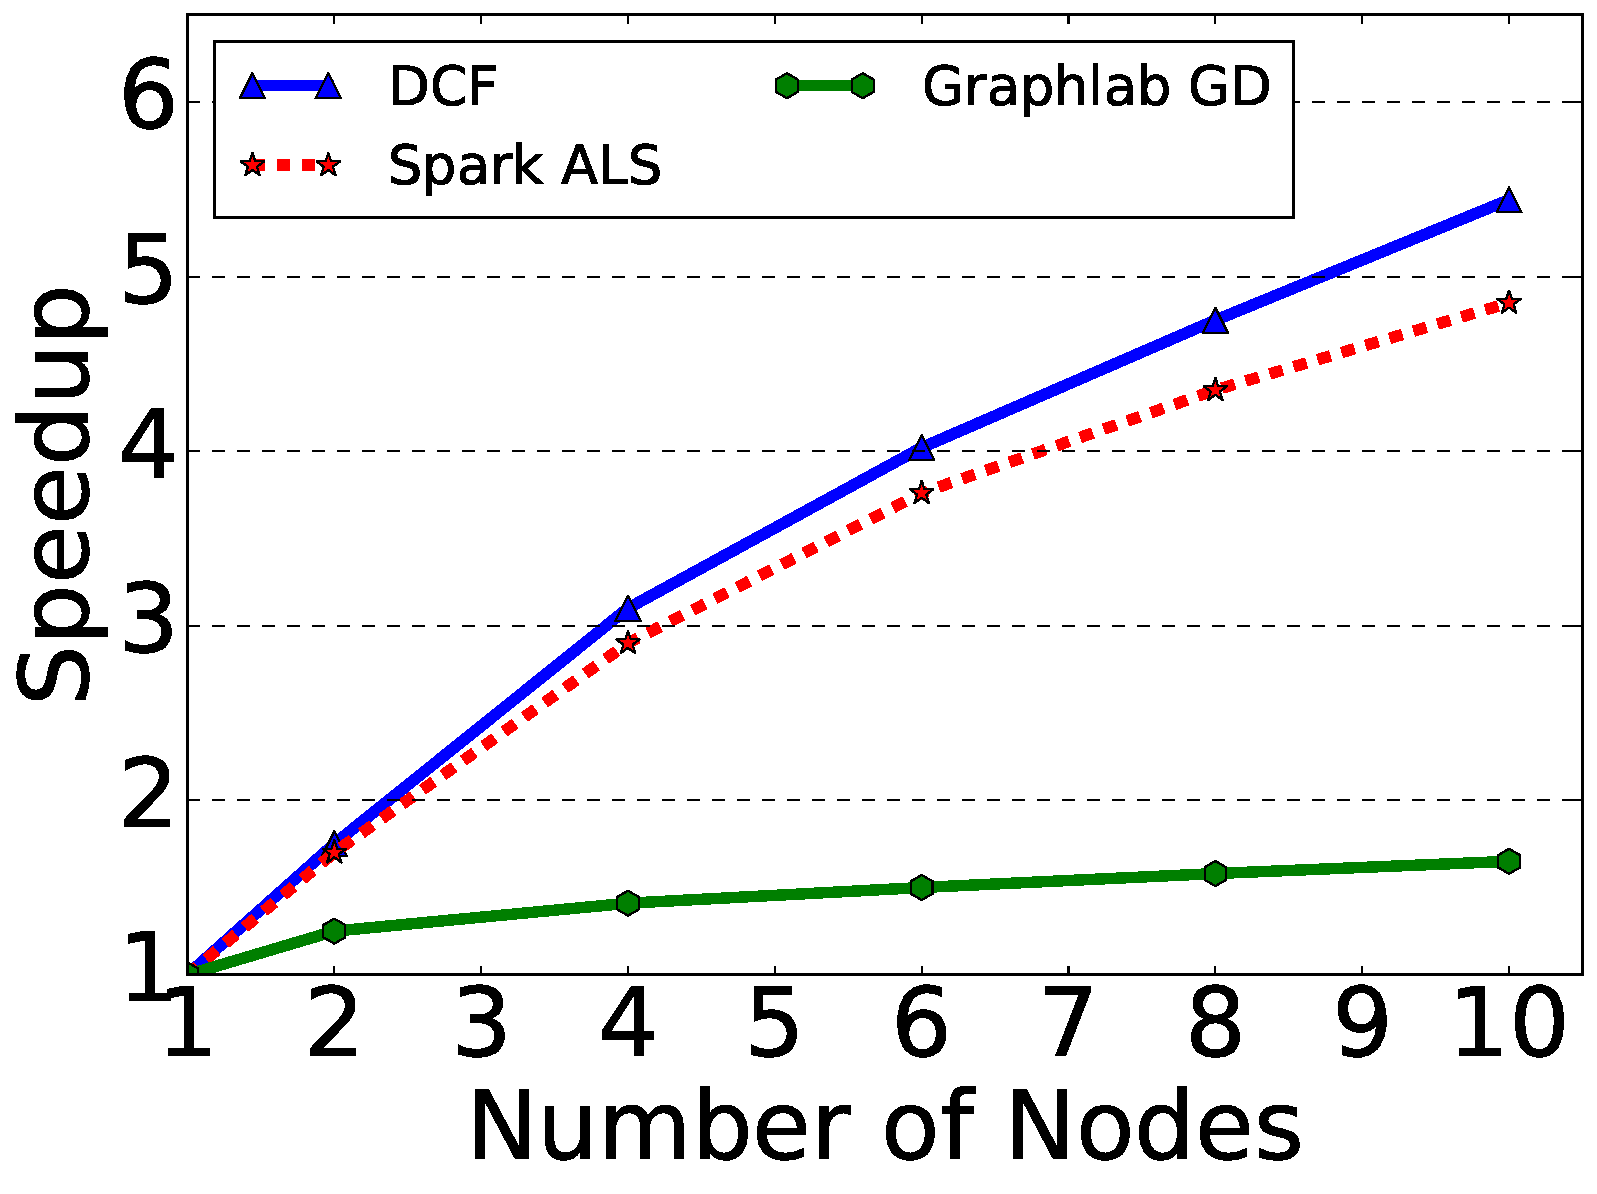
\includegraphics[width=2.5in]{pics/node.pdf}
%\caption{Speedup Comparisons of Three Algorithms in Distributed System}
%\vspace{-15pt}
%\label{fig:node}
%\end{figure}
\vspace{-15pt}
\subsection{Scalability}
%\vspace{-5pt}
\label{sub:sca}

In the last subsection, we evaluate the scalability of DCF in comparison with Spark ALS and Graphlab GD. The evaluation of the three algorithms is conducted on multicore system and distributed system. Yahoo Music has the largest rating size, which leads to high computation and communication load, so we select it as the dataset for this experiment. As shown in left part of Figure \ref{fig:core}, DCF has a near linear scalability when the core number increases, and achieves a speedup of 7.45 on 10 cores. ALS has similar scalability with DCF and achieve a speedup of 6.87 on 10 cores. Graphlab GD has the worst scalability and only achieve a speedup of 1.9 on 10 cores.

In distributed system, we evaluate the scalability on 10 nodes. As shown in right part of Figure \ref{fig:core}, DCF achieves a speedup of 5.44 on 10 nodes, and ALS has similar speedup of 4.85. Graphlab GD also shows the worst scalability on nodes and only achieves a speedup of 1.65 on 10 nodes.

In conclusion, DCF shows the best scalability in three algorithms and has superior performance in both multicore system and distributed system.

\vspace{-10pt}
\section{Related Work}
\label{sec:relatedWork}
\vspace{-5pt}
In recent years, parallel researches on collaborative filtering are developing parallel algorithms for ALS and gradient descent. Mahout, the machine learning library for Hadoop \cite{Hadoop}, implemented model based algorithms with MapReduce \cite{MapReduce} computation model. Spark \cite{SparkMllib} implemented ALS \cite{SparkCF} and utilized its Dataframe \cite{dataFrame}  data structure to improve the performance. However, high computation complexity of ALS becomes the bottleneck of these systems.

In order to achieve higher performance, many studies focus on parallel gradient descent algorithm for its low computation complexity feature. Graphlab \cite{graphlab}, a distributed asynchronous system, provided asynchronous gradient descent. Due to massive data movements between nodes, graphlab shows low performance in large dataset because of the network bottleneck.
In recent years, parameter server architecture were proposed to support distributed gradient descent. STRADS \cite{strads} in Petuum was proposed to schedule model parallel machine learning algorithms on distributed platform. Parameter Server \cite{ps} proposed bounded synchronous technique and several network optimizations to support gradient descent. As for these parameter sever architecture based systems, the task scheduling level is on data partition but not on key-value pair. Tensorflow \cite{tensorflow}, another dataflow inspired system, only adopted pipelining feature of dataflow model to support gradient descent. As for parallel collaborative filtering studies \cite{sgdFast2015} \cite{sgdKdd2015} \cite{StarPU}, They mainly focused on multicore system but not distributed system.
\vspace{-15pt}
\section{Conclusion}
\label{sec:conclusion}
\vspace{-5pt}
Dataflow model is a natural parallel model which can exploit maximum
parallelism of algorithms by analyzing data dependency to asynchronously
execute tasks in runtime execution. At present, recommender
systems are facing challenges of the increasing rating size and low performance of current big data systems. We design and implement dataflow based collaborative filtering (DCF) algorithm to improve the performance. We propose three optimizations (dummy edge, multicasting and mini-bach) to further improve our design by avoiding fine-grain overhead and reducing computation and data movements. The experiment results illustrate that DCF can significantly improve the performance on distributed system.

\vspace{-10pt}
\bibliographystyle{splncs03}
\bibliography{ref}
\vspace{-20pt}


\end{document}
